\documentclass[journal]{IEEEtran}

\usepackage{graphicx,subfigure}
\usepackage{booktabs}
\usepackage{textcomp}
\usepackage{acronym}
\usepackage{enumitem}
\usepackage{array}
\newcolumntype{C}[1]{>{\centering}m{#1}}
\usepackage{amsmath}
\usepackage{amssymb}
\usepackage{color}
\usepackage{amsfonts}
\usepackage{psfrag}
\usepackage[justification=centering]{caption}
\hyphenation{op-tical net-works semi-conduc-tor}
\usepackage[algoruled]{algorithm2e}
\renewcommand{\ss}{\resizebox{4pt}{2pt}{$\square$}}

%\makeatletter
%\def\endthebibliography{%
%	\def\@noitemerr{\@latex@warning{Empty `thebibliography' environment}}%
%	\endlist
%}
%\makeatother

\newacro{CFR}{channel frequency response}
\newacro{PLC}{power line communication}
\newacro{ACG}{average channel gain}
\newacro{CB}{coherence bandwidth}
\newacro{ACA}{average channel attenuation}
\newacro{RMS-DS}{root mean squared delay spread}
\newacro{CT}{coherence time}
\newacro{CIR}{channel impulse response}
\newacro{DFT}{discrete Fourier transform}
\newacro{HS-OFDM}{Hermitian Symmetric Orthogonal Frequency Division Multiplexing}
\newacro{BPSK}{binary phase shift keying}
\newacro{r.va.}{random variables}
\newacro{CP}{cyclic prefix}
\newacro{SFO}{sampling-frequency offset}
\newacro{MLE}{Maximum Likelihood Estimation}
\newacro{AIC}{Akaike information criterion}
\newacro{BIC}{Bayesian information criterion}
\newacro{EDC}{Efficient determination criterion}
\newacro{LPTV}{linear periodically time varying}
\newacro{LTI}{linear time-invariant}
\newacro{OFDM}{Orthogonal Frequency Division Multiplexing}
\newacro{IFT}{inverse Fourier transform}
\newacro{r.v.}{random vector}
\newacro{WLC}{wireless communication}
\newacro{IoT}{Internet of Things}
\newacro{SG}{smart grid}
\newacro{RF}{radio frequency}
\newacro{WLAN}{wireless local area network} 
\newacro{LPWAN}{Low Power Wide Area Networks}
\newacro{UWB}{Ultra-wide-band}
\begin{document}

\title{Statistical Modeling of Frequency Responses of the Brazilian In-Home Channels: PLC and Cascade of PLC and Wireless}

\author{Thiago~F.~do~A.~Nogueira,~Guilherme~R.~Colen,~\IEEEmembership{Member,~IEEE},
	~Victor~Fernandes,~and~Moises~V.~Ribeiro,~\IEEEmembership{Senior~Member,~IEEE}
\thanks{T. F. do A. Nogueira (thiago.nogueira@engenharia.ufjf.br), G. R. Colen (guilherme.colen@engenharia.ufjf.br), and V. Fernandes (victor.fernandes@engenharia.ufjf.br) are with the Electrical Engineering Department, Federal University of Juiz	de Fora (UFJF), Juiz de Fora 36036-330, Brazil.}
\thanks{M. V. Ribeiro (mribeiro@ieee.org) is with the Electrical Engineering
	Department, Federal University of Juiz de Fora (UFJF), Juiz de Fora 36036-330, Brazil and Smarti9 LTD., Juiz de Fora 36036-330, Brazil.}}

% The paper headers
%\markboth{Journal of \LaTeX\ Class Files,~Vol.~14, No.~8, August~2015}%
%{Shell \MakeLowercase{\textit{et al.}}: Bare Demo of IEEEtran.cls for IEEE Journals}

\maketitle

\begin{abstract}
%This paper focuses on statistical characterization and modeling of frequency responses of the Brazilian in-home power line channels based on a data set, which was acquired through a measurement campaign carried out in seven Brazilian residences, comprising the frequency band from $1.7$ up to $100$~MHz. In this regard, a procedure to obtain the statistical models in the aforementioned frequency bandwidth is detailed. Based on the use of four distinct criteria, the best statistical distributions that model each one of the magnitude and phase of the channel frequency response estimates are addressed. In addition, we discuss the use of an interpolation technique based on cubic Splines for yielding the representation of the statistical distributions' parameters in the continuous time domain. Numerical and analytical results showed that the Beta and Uniform distributions are the best statistical distributions for modeling the magnitude and phase functions, respectively, of the frequency response of the Brazilian in-home power line channels. Moreover, the parameters of the Beta distribution are shown to be dependent upon the frequency tone while the parameters of the Uniform one are frequency independent. Finally, a statistical modeling of magnitude and phase functions in the continuous-time domain is introduced.  

\end{abstract}

\begin{IEEEkeywords}
Statistical characterization, power line communication, measurement campaign, in-home broadband channels, channel frequency response.
\end{IEEEkeywords}

\IEEEpeerreviewmaketitle

\section{Introduction}

%\IEEEPARstart{P}{ower} line communication (PLC\acused{PLC}) systems have been investigated by academic and industry sectors worldwide over the past decades. Recently, these systems have become attractive solutions for data communication once they can be deployed over the existing electric power systems infrastructure. As a matter of fact, the ubiquitousness of electric power systems is the main advantage associated with the use of \ac{PLC} technologies. Based on this very important characteristic, \ac{PLC} systems can assist the deployment of \ac{SG}, the \ac{IoT}, smart city, and Industry $4.0$ technologies. On the other hand, one may say that the wireless communications constitute a more established alternative for this purpose due to its low-cost and suitability for fulfilling the needs and demands of these technologies. However, it is widely recognized that \ac{SG}, \ac{IoT}, smart city and Industry $4.0$ will be supported by a heterogeneous set of telecommunication technologies, as no single solution fits all scenarios \cite{Galli2011}. For the given reasons, \ac{PLC} and unlicensed wireless communications are considered as the two leading data communication technologies for \ac{SG} applications and \ac{IoT} \cite{Sayed2014, Dib, Sayed2015}. 
%
%Some researches have pointed out that the deployment and operational costs related to the \ac{PLC} systems can be low \cite{Hrasnica:PLC_design, Dib} and it constitutes a relevant advantage in favor of these data communication systems; however, electric power grids were originally conceived and designed for generating, transmitting and delivering or distributing energy to consumers or prosumers and, as a consequence, the propagation of signals carrying information through power lines may suffer severe attenuation and/or frequency-selective fading due to the use of non-ideal and unshielded conductors, the existence of impedance mismatching, and dynamics of loads and equipments connected to electric power grids. Also, it is important to highlight that signals carrying information over power line can be corrupted by the high power impulsive noise presences associated with the dynamics of electric power systems and the use of electromagnetically unshielded power lines. In addition, the diversity of topologies and distances of electric power grids may result in very disparate behaviors that demand powerful \ac{PLC} systems for dealing with this problems; power lines work as antennas and, as consequence, interference with other telecommunication systems operating in the same frequency band may result in significant \ac{RF} interference; and the remarkable increase of connections of new types of loads make the electric power grids a challenging media for data communication purposes. Moreover, it is important to pay attention to the voltage level (low, medium and high-voltage), the type of environment, such as indoor (vehicle, residences and building) and outdoor (metropolitan and rural areas), among other issues.
%
%As a common sense in the telecommunication field, it is well-established that the measurement, characterization and modeling of \ac{PLC} channels are mandatory tasks to be \textit{a priori} accomplished for fostering advances in \ac{PLC} systems because they yield important information for driving the designers of telecommunication devices. Due to the complexity and diversity of electric power systems, it is well-accepted by the \ac{PLC} community that \ac{PLC} channels can be, in terms of voltage level, organized in the low-voltage (indoor or outdoor) \cite{Zhai:low}, medium-voltage (outdoor and underground) \cite{Lazaropoulos} and high-voltage (outdoor) \cite{Zajc}. It is important to emphasize that this organization is aligned with the electric power systems field. Also, it deserves attention the fact that the underground medium-voltage electric power grids are more distinct because of the surrounding environment \cite{Aquilue}. 
%
%Focusing on the electric power grids located in indoor facilities, research efforts toward the characterization and modeling of \ac{PLC} channels may be organized in terms of the type of facilities as follows: residential or commercial buildings, known as in-home or in-building \ac{PLC} \cite{Amirshahi:PLC,Tlich:Indoor} and in-vehicles (i.e., cars \cite{Vallejo:Vehicle_PLC}, ships \cite{Barmada:Ships_PLC}, and aircrafts \cite{Jones:Aircraft_PLC,Andrei:Meas,Andrey2016}). Regarding the frequency band of operation, the \ac{PLC} community does not follow the communications community once the concept of the narrowband-\ac{PLC} systems is associated with data communication through the frequency band delimited by $0$ and $500$~kHz \cite{Gassara:Charac_PLC,Chrysochos:MIMO_OFDM}, while the concept of the broadband-\ac{PLC} systems refers to the use of the frequency band from $1.705$ up to $100$~MHz \cite{Tlich:Indoor,Galli:Wireline}, depending on the telecommunications regulation, for data communication purpose. For instance, in Brazil, broadband-\ac{PLC} systems are allowed to operate in the frequency band delimited by $1.7$ and $50$~MHz \cite{Anatel:PLC}. Some contributions point out that the frequency band between $0$ and $500$~MHz may be used by future generation of \ac{PLC} systems \cite{Luis:doc,zeddam1}. In this context, several improvements are being investigated, such as those obtained by cooperative communication \cite{mateus:2018,Michelle2016,Roberto2015}. 
%
%Still addressing the indoor electric power grids and focusing on the in-home environments, several contributions related to research efforts for \ac{PLC} channels characterizations carried out in distinct countries can be highlighted. For instance, \cite{Canete:Model} discussed in-home \ac{PLC} channels in Spain that are related to channel attenuation and additive noise in the frequency band between $1.705$ and $30$~MHz, while \cite{Canete:PLC} considered other features, such as delay spread, \ac{ACG} and \ac{CB}. Also, \cite{Cortes:PLC} discussed the normal/log-normal nature of delay spread and \ac{ACG}. In \cite{GalliUS,Galli:Wireline}, the in-home \ac{PLC} channels in some urban and suburban United States (US) residences were characterized in terms of \ac{ACG} and \ac{RMS-DS}, considering the frequency band ranging from $2$ up to $30$~MHz. In \cite{Tlich:Indoor}, a characterization of in-home \ac{PLC} channels was performed in some urban and suburban France residences, describing values of \ac{CB} and time-delay parameters, considering the frequency band ranging from $30$~kHz up to $100$~MHz. Recently, \cite{Thiago:Characterization} has analyzed the \ac{CFR}, \ac{ACA}, \ac{RMS-DS}, \ac{CB}, and \ac{CT} of Brazilian in-home \ac{PLC} channels when the frequency band ranges from $1.7$ up to $100$~MHz. Analyzing the aforementioned works and contributions, we notice that several works had adopted as true that the Log-normal distribution for modeling the \ac{CFR} magnitude; however, the lack of confidence on it \cite{Cortes:PLC} brings our attention to the necessity of further investigation of \ac{CFR} of in-home \ac{PLC} channels.
%
%Concerning \ac{WLC}, it is important to point out the high dependence on line-of-sight propagation, the increasing signal attenuation along with both distance and carrier frequency, the susceptibility to interference among two or more telecommunication systems operating in the same frequency band, the scarcity of spectrum, and vulnerability to non-authorized access, among other things, constitute a relevant set of problems. Also, the transmitted signal through the air suffers three different propagation effects: reflection, scattering and diffraction \cite{Guze}. Remarkable problems in \ac{WLC} are associatated with the distortions introduced by the aforementioned propagation effects and co-channel interference, which is primarily generated from uncoordinated transmissions \cite{Sayed2015}.  
%
%\ac{WLC} channel characterization and modeling has been atracting high attention since they can highly reduce the time of developing \ac{WLC} systems. The \ac{WLC} system support several different technologies and includes, among others, the \ac{WLAN}, comprising five distinct frequency bands: $900$~MHz, $2.4$~GHz, $3.6$~GHz, $5$~GHz, and $60$~GHz \cite{IEEEWI}; the cellular data service, using the main frequency range around $900$~MHz, $1.8$~GHz and $1.9$~GHz \cite{GSM}; the \ac{LPWAN}, which bridges the frequency gap between \ac{WLAN} and cellular technologies, commonly used on \ac{IoT} applications \cite{Patel}. As the number of users and service stations has significantly increased in the last decades, more research efforts to correctly characterize and model \ac{WLC} channel have been carried out. Channel characterization and modeling in such situations can give valuable insights such as predicting the communication quality of a \ac{WLC} system when high data traffic and or large number of users are demanding the same frequency bandwidth. Among the well established \ac{WLC} channel models in the literature we can mention: the COST 2100 channel model \cite{COST}, that provides statically close-to-true descriptions of wireless channels both for indoor scenarios, regarding $3.6$ and $5.3$~GHz frequency bands, and outdoor scenarios, covering the $400$~MHz frequency band; the IEEE 802.15.4a channel model \cite{802.15}, concerning models for diverse frequency ranges and environments, such as indoor and outdoor \ac{UWB} channels covering the frequency range from $2$ up to $6$ GHz; the Hiperlan$/2$ channel model \cite{Hiperlan2}, covering wireless models in different indoor scenarios for the frequency band of $5$~GHz. Regarding the single-input single-output modeling of \ac{WLC} channels, it is worth stating that the frequency band up to $6$~GHz has been very well investigated for characterization and modeling purpose, while the research efforts related related to multiple-input multiple-output is somehow well-established. Currently, a great deal of attention is toward the frequency band related to $5$~GHz and beyond.
%
%In a nutshell, it is important to emphasize that \ac{PLC} and \ac{WLC} media present distinct characteristics that can be jointly exploited for improving the telecommunication systems performance in terms of reliability, data-rate, physical layer security, coverage, and flexibility in the physical and link layers \cite{Dib,Victor2017,Sayed2015,Holden2011}. In this regard, a hybrid approach exploiting the existing diversity between \ac{PLC} and \ac{WLC} communication systems was initially introduced in order to overcome the problems experienced in both isolated systems. Essentially, it assumes that the \ac{PLC} and \ac{WLC} channels are concatenated in series such that \ac{PLC} and \ac{WLC} devices operate in the same frequency band. This type of hybrid data communication system emerged at the very beginning of the XX Century \cite{Mischa} but the advances related to \ac{WLC} system during the following decades drastically reduced the interests in this kind of data communication. Only at the beginning of the XXI Century, precisely one century after its initial investigation, \cite{thiago:hyb} revisited and investigated this kind of channels. As it was initially proposed, it made use of unshielded power lines to propagate and irradiate the transmitted signal by a \ac{PLC} device. In other words, it assumes that the power line acts as an antenna. As a result, the power lines radiate signals and, conversely, wireless signals, generated by a \ac{WLC} device, are inductively injected into the power lines. Currently, there is a great deal of attention in parallel and cascade usages of \ac{PLC} and \ac{WLC} channels to provide either reliability or high data rate. The former approach result in the so-called the hybrid \ac{PLC}/\ac{WLC} system while the later is coined the hybrid \ac{PLC}-\ac{WLC} system. The hybrid \ac{PLC}/\ac{WLC} system have also been investigated as an alternative to improve data communication performance \cite{Victor2017,Sayed2014} since it can take advantage of both electric power grids and air to improve data rate and reliability between source and destination nodes under several circumstances, see \cite{Dib} for details. In such data communication systems, electric power grids and wireless media are used simultaneously in a cooperative perspective to maximize the available channel resources and, as a consequence, to fulfill data communication constraints.
%
%At this time, it is important to emphasize that there are several works for characterizing \ac{PLC} channels but \ac{PLC} channel modeling is still an open problem, once the behavior of electric power grids over narrowband (frequency band from $0$ up to $500$~kHz) and broadband (frequency band from $1.7$ up to $100$~MHz) are different in terms of signal propagation and additive noise influence due to the complexity of electric power systems (e.g., load dynamics, topologies and voltage levels). Therefore, channel modeling is still an open problem related to \ac{PLC} systems. Regarding \ac{WLC} channels, the huge research efforts carried out worldwide have introduced representative models that are well-established in the literature \cite{COST,802.15,Hiperlan2}. Furthermore, when the discussion is toward to hybrid \ac{PLC}-\ac{WLC} channels, which is defined as the series concatenation of \ac{PLC} and \ac{WLC} channels, there is a complete lack of contribution regarding their modeling in the literature. In other words, the investigation of channel models for \ac{PLC} channels and hybrid \ac{PLC}-\ac{WLC} channels is an important research endeavor demanding attention. In this regard, this dissertation strives to cover this gap an to expand the knowledge on these channels by extracting and modeling the benefits of \ac{PLC} and hybrid \ac{PLC}-\ac{WLC} channels for data communication in the frequency band delimited by $1.7$ and $100$~MHz.
%
%Aiming to pay attention to \ac{PLC} and hybrid \ac{PLC}-\ac{WLC} channels for data communication, this thesis seek to provide statistical characterization and modeling of \acp{CFR} of Brazilian in-home \ac{PLC} and hybrid \ac{PLC}-\ac{WLC} channels, in order to support future efforts for simulating and designing in-home data communication systems. In this context, an enhanced statistical modeling method, which emerged from the drawbacks associated with the methodology presented in \cite{Luis:AI,Luis:doc}, is proposed. Furthermore, the statistical characterization and modeling results, based on data sets of measured \acp{CFR} of in-home \ac{PLC} and hybrid \ac{PLC}-\ac{WLC} channels, are detailed.
%The mentioned data sets were acquired during a measurement campaign performed in several Brazilian residences, see more informations about the measurement campaign in \cite{Thiago:Characterization,thiago:hyb,thiago:hyb2,thiago:doc}. In this contribution, the frequency band is set to be from $1.7$ up to $100$~MHz, once it covers broadband \ac{PLC} systems that can offer data rates in the order of $1-2$~Gbps \cite{Galli:indoor,Thiago:Characterization}. Also, it is a frequency band that comprises Brazilian, European and US telecommunication regulations for \ac{PLC} systems. Overall, the main objectives of this thesis may be organized as follows:
%
%\begin{itemize}
%	\item To introduce the enhanced statistical modeling method, based on the method presented in \cite{Luis:AI,Luis:doc}, that is capable of searching for the best statistical distribution to model the \ac{CFR} of in-home \ac{PLC} and hybrid \ac{PLC}-\ac{WLC} channels. It treats the magnitude and phase components of \acp{CFR} as random processes. Based on the fact that the proposed enhanced statistical modeling method is designed in the discrete-time domain, it encompasses a procedure for interpolating the parameters values of the chosen statistical distributions, by dividing the desired frequency band into subbands and using the cubic Spline interpolation technique to come up with a concise representation (i.e., finite and low number of parameters) of the parameters of this random process in the continuous-frequency domain. Also, the algorithms that implements the enhanced statistical modeling method is detailed. 
%	
%	\item To provide statistical analyses of measured Brazilian in-home \ac{PLC} and hybrid \ac{PLC}-\ac{WLC} channels, which were acquired by a measurement campaign carried out several residences and took into account the frequency band between $1.7$ and $100$~MHz. To present the models of such channels and to compare the attained results with the ones found in the literature regarding \ac{PLC} channels. To introduce, for the first time, models of the \acp{CFR} of hybrid \ac{PLC}-\ac{WLC} channels. 
%\end{itemize}

%%%%%%%%%%%%%%%%%%%%%%%%%%%%%%%%%%%%%%%%

%\IEEEPARstart{P}{ower} line communication (PLC\acused{PLC}) systems have been investigated by academic and industry sectors worldwide over the past decades. Recently, these systems have became attractive solutions for data communication once they can be deployed over the existing electric power systems' infrastructure. As a matter of fact, the ubiquitousness of electric power systems is the main advantage associated with the use of \ac{PLC} technologies. Based on this very important characteristic, \ac{PLC} systems can assist the deployment of Smart Grids, Internet of Things and Industry $4.0$ technologies. 
%
%Some researches have pointed out that the deployment and operation costs related to \ac{PLC} systems can be low \cite{Hrasnica:PLC_design, Dib} and it constitute a relevant advantage in favor of these systems; however, electric power grids were not originally designed for data communication purposes and, as a consequence, the propagation of information carrying signals through power lines may suffer severe attenuation and/or frequency-selective fading due to the use of non-ideal conductors and the existence of impedance mismatchings. Also, these signals can be corrupted by the high power impulsive noise presence associated with the dynamics of electric power systems and the use of electromagnetically unshielded power lines. In addition, the diversity of topologies of electric power grids and the fact that power lines can be seen as antennas and, as consequence, may suffer significant influence from the RF signals, make the electric power grids a challenging media for data communication purposes.  
%
%It is well-established in the communications literature that the characterization and modeling of \ac{PLC} channels are mandatory tasks to be \textit{a priori} accomplished for fostering advances in \ac{PLC} systems. In this context, the \ac{PLC} channels can be organized in the low-voltage (indoor or outdoor) \cite{Zhai:low}, medium-voltage (outdoor and underground) \cite{Lazaropoulos} and high-voltage (outdoor) \cite{Zajc}. Among them, the underground medium-voltage \ac{PLC} systems are more distinct because of the environment conditions \cite{Aquilue}. Focusing on the indoor electric power grids, recent research efforts toward the characterization and modeling of \ac{PLC} channels may be organized as follows: residential or commercial buildings, known as in-home or in-building \ac{PLC} \cite{Amirshahi:PLC,Tlich:Indoor} and in-vehicles (i.e., cars \cite{Vallejo:Vehicle_PLC}, ships \cite{Barmada:Ships_PLC}, and aircrafts \cite{Jones:Aircraft_PLC}). Regarding the frequency band of operation, the \ac{PLC} community does not follow the communications community because the concept of the narrowband-\ac{PLC} systems is associated with the frequency band delimited by $0$ and $500$~kHz \cite{Gassara:Charac_PLC,Chrysochos:MIMO_OFDM}, while the concept of the broadband-\ac{PLC} systems cover the frequency band from $1.705$ up to $100$~MHz \cite{Tlich:Indoor,Galli:Wireline}, depending on the telecommunications regulation. For instance, broadband-\ac{PLC} systems are allowed to operate in the frequency band delimited by $1.7$ and $50$~MHz \cite{Anatel:PLC}.
%
%Still addressing the indoor electric power grids and focusing on the in-home environments, some few contributions related to distinct countries can be highlighted. For instance, \cite{Canete:Model} discussed in-home \ac{PLC} channels in Spain that are related to channel attenuation and additive noise in the frequency band between $1.705$ and $30$~MHz, while \cite{Canete:PLC} considered other features, such as delay spread, \ac{ACG} and \ac{CB}. Also, \cite{Cortes:PLC} discussed the normal/log-normal nature of delay spread and \ac{ACG}. In \cite{GalliUS,Galli:Wireline}, the in-home \ac{PLC} channels in some urban and suburban United States (US) residences were characterized in terms of \ac{ACG} and \ac{RMS-DS}, considering the frequency band ranging from $2$ up to $30$~MHz. In \cite{Tlich:Indoor} a characterization of in-home \ac{PLC} channels was performed in some urban and suburban France residences, describing values of coherence bandwidth and time-delay parameters, considering the frequency band ranging from $30$~kHz up to $100$~MHz. Recently, \cite{Thiago:Characterization} has analyzed the \ac{CFR}, \ac{ACA}, \ac{RMS-DS}, \ac{CB}, and \ac{CT} of Brazilian in-home \ac{PLC} channels when the frequency band ranges from $1.7$ up to $100$~MHz. Analyzing the aforementioned works and contributions, we notice that several works have adopted as true that the Log-normal distribution for modeling the \ac{CFR} magnitude; however, the lack of confidence on it, see \cite{Cortes:PLC}, brings our attention to the necessity of further investigation of \ac{CFR} of in-home \ac{PLC} channels. 
%
%Aiming to bring more information about the aforementioned issue, the main objective of this paper is to provide a statistical characterization and modeling of \ac{CFR} of Brazilian in-home \ac{PLC} channels in order to support future efforts for simulating and designing in-home \ac{PLC} systems within a worldwide perspective. The statistical characterization and modeling is based on the data set of measured \ac{CFR}s of in-home \ac{PLC} channels, which were acquired during a measurement campaign performed in several Brazilian residences, see details about the measurement campaign in \cite{Thiago:Characterization}. In this contribution, the frequency band is set to be from $1.7$ up to $100$~MHz, once it represents a tendency for future \ac{PLC} systems due to the achievable data rate on the order of $1-2$~Gbps \cite{Galli:indoor,Thiago:Characterization}. The main contributions of this work are summarized as follows:
%
%\begin{itemize}
%	\item Introduction of an useful and simple  method that is capable of searching for the best statistical distribution to model the \ac{CFR} magnitude and phase functions of in-home \ac{PLC} channels. This method also encompass a procedure for interpolating the parameters values of the chosen statistical distributions, using the cubic Spline interpolation technique.
%	
%	\item Statistical analyses of measured in-home \ac{PLC} channels in the frequency band from $1.7$ up to $100$~MHz for obtaining the parameters of the statistical distributions. This frequency band comprises Brazilian, European, and US telecommunication regulations for \ac{PLC} systems. 
%    \end{itemize}
%
%Based on the numerical analyses, the following findings may be brought to attention:
%
%\begin{itemize}
%	\item The magnitude function of the \ac{CFR}s of Brazilian in-home \ac{PLC} channels is better modeled by the Beta distribution assuming the frequency band from $1.7$ up to $100$~MHz. The parameters of this statistical distribution depends upon the value of the frequency tone. In other words, the magnitude is a non-stationary random process. 
%   \item The use of a technique based on cubic Spline for interpolating the parameters of the statistical distribution associated the \ac{CFR} over the considered frequency band results in a simple modeling if the frequency ranges in the real set. 
%	\item The phase function of the \ac{CFR}s of Brazilian in-home \ac{PLC} channels is better modeled by the Uniform distribution for the frequency band from $1.7$ up to $100$~MHz. Statistical results have shown that the adoption of this distribution is independent of the chosen frequency. In other words, the phase is a stationary random process. 
%\end{itemize}
%
%The remainder of this paper is structured as follows: Section II addresses
%the problem formulation; Section III describes the methodology to obtain the uncorrelated \ac{CFR} model, while Section IV discusses the statistical analyses and results of the proposed methodology to model the \ac{CFR} of \ac{PLC} channels. Finally, the paper conclusions are summarized in Section V.

%%%%%%%%%%%%%%%%%
%The findings reported in \cite{thiago:hyb,thiago:hyb2,thiago:doc} are very interesting to motivate this kind of data communication systems for fulfilling the scarcity of spectrum for dealing with te astonishing increase of data exchanges among entities in smart grids, the \ac{IoT} and industry $4.0$ applications. Advances in this field may facilitate the work of researchers and hybrid \ac{PLC}-\ac{WLC} systems designers under the availability and representative of hybrid \ac{PLC}-\ac{WLC} channels. 

\section{Problem Formulation}

Fig. \ref{PLCchannel} portrays the block diagram of a \ac{PLC} system which is supposed to transmit information carrying signals through an electric power circuit in the frequency band delimited by $0$ and $B$~Hz (i.e., baseband data communication). This electric power circuit is supposed to be linear and time-varying system. According to this figure, the received signal is expressed as
\begin{equation} \label{received signal}
Y_P(t) = \tilde{Y}_P(t)+V_P(t) = \int_{-\infty}^{+\infty} h_P(t,\tau) X(\tau) d\tau + V_P(t),
\end{equation}
where $X(t)\in \mathbb{R}$ is the transmitted signal modeled as a wide sense stationary stochastic process; $h_P(t,\tau)\in \mathbb{R}$ is the time varying \ac{CIR}, related to an impulse applied on the \ac{PLC} channel at the instant $\tau$, modeling the propagation of the transmitted signal through the electric power circuit; $V_P(t)\in \mathbb{R}$ is the additive noise that is modeled as a wide sense stationary random process, $\tilde{Y}_P(t)\in \mathbb{R}$ and $Y_P(t)\in \mathbb{R}$ denote wide sense stationary random processes called the free-of-noise received signal and the received signal, respectively.

\begin{figure}[h]
	\centering
	\psfrag{A}[c][c][1]{Transmitter}
	\psfrag{B}[c][c][1]{PLC Channel}
	\psfrag{C}[c][c][1]{Receiver}
	\psfrag{D}[c][c][1]{$T_X$}
	\psfrag{E}[c][c][1]{$X(t)$}
	\psfrag{F}[c][c][1]{$h_P(t,\tau)$}
	\psfrag{G}[c][c][1]{$\tilde{Y}_P(t)$}
	\psfrag{H}[c][c][1]{$V_P(t)$}
	\psfrag{I}[c][c][1]{$Y_P(t)$}
	\psfrag{J}[c][c][1]{$R_X$}
	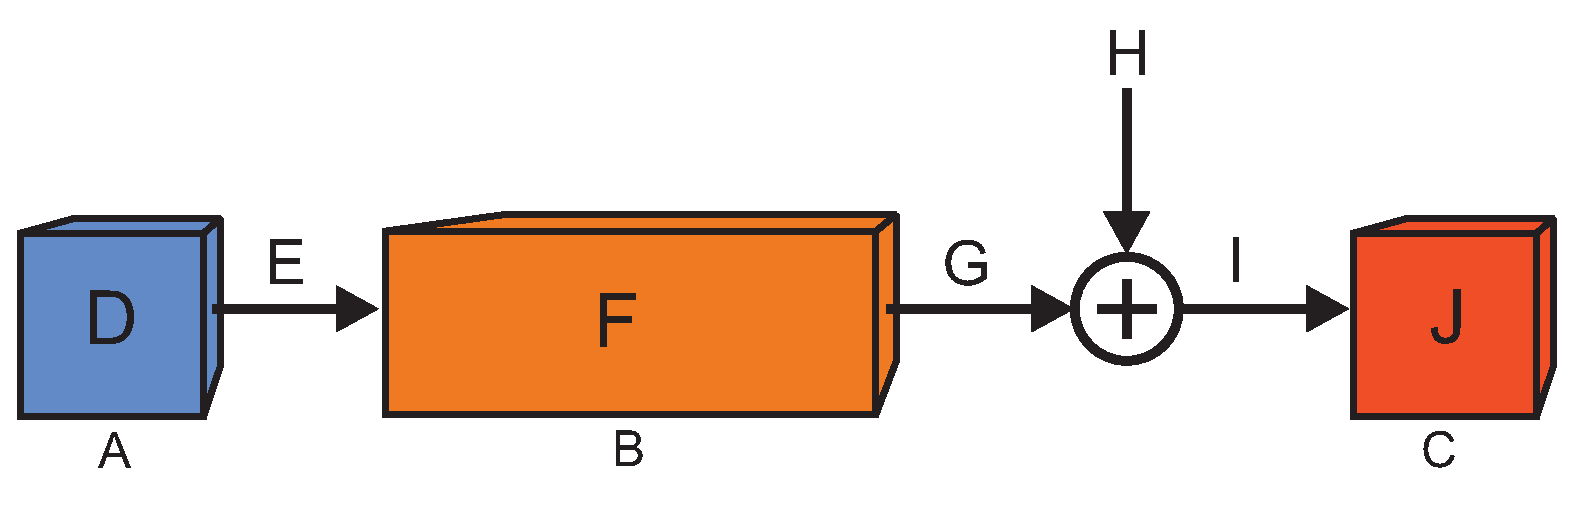
\includegraphics[width=0.49\textwidth]{images/PLCchannel.eps}
	\caption{The block diagram of a PLC system.}
	\label{PLCchannel}
\end{figure}

Due to the \ac{LPTV} behavior of \ac{PLC} channels, $h_P(t,\tau)$ can be considered as a cyclostationary stochastic random process with a period equal to a half of the mains frequency \cite{Colen:TCRA}. Based on the knowledge of the coherence time, $T_c \in \mathbb{R}_+$, of the \ac{PLC} channels, the mains cycle ($50$~Hz or $60$~Hz) can be divided into microslots of time interval duration equal to $T_m\in \mathbb{R}_+|T_m < T_c$ and, as a consequence, the \ac{PLC} channels can be modeled as \ac{LTI} during the time interval duration of one microslot. In other words, the channel impulse response of a \ac{PLC} channel at the $i^{th}$ microslot can be expressed as
\begin{equation} \label{discreteh}
h_{i}(t),~\forall~t \in [iT_{m}, (i+1)T_{m}] \mid T_{m} < T_{c}.
\end{equation}
From now on, we drop the index $i$ for facilitating further deductions. Based on this adoption, the discrete-time representation of the \ac{CIR} of the \ac{PLC} channel in a microslot is given by
\begin{equation} \label{discreteCFR}
h[n] = h_P(t)|_{t=nT_s} , n = 0,1, \ldots, L_h-1, 
\end{equation}
where $L_{h}$ is the length of the \ac{LTI} \ac{PLC} channel, $T_s=1/f_s$ is the sampling period and $f_s=2B$~Hz is the sampling frequency. Usually, the value of $L_{h}$ contribute to the adoption of an \ac{HS-OFDM} scheme for channel estimation once the number of subcarriers of an \ac{HS-OFDM} symbol ($2N$) is chosen to ensure that $2N \gg L_h$. Moreover, $B/N < B_c$, in which $B_c$ is the coherence bandwidth of the \ac{PLC} channels. In order to work with $2N$ subcarriers in the \ac{HS-OFDM} scheme for performing \ac{CFR} estimation, the zero-padding have to be applied to $\{h[n]\}$. In vectorial terms, let ${\bf h}=[h_0 h_1 \ldots h_{L_h-1}]^T$, such as $h_n=h[n]$, then we can obtain an $2N\text{-length}$~vector (i.e., $N\in \mathbb{N}|B/N<B_c$) that represents the extended version of the vector ${\bf h}$ when the zero-padding approach is taken into account. As a consequence, the vectorial representation of the \ac{CFR} associated with the extended version of the vector $\mathbf{h}$ is expressed as
\begin{equation}
\mathbf{H} = \mathbf{W}_{2N}  \begin{bmatrix} \mathbf{I}_{L_h} \\ \mathbf{0}_{(2N-L_{h})\times L_{h}} \end{bmatrix} \mathbf{h},
\end{equation}
where $\mathbf{W}_{2N} \in \mathbb{C}^{2N\times 2N}$ denotes the $2N \times 2N$-size \ac{DFT} matrix, $ \mathbf{I}_{L_h} \in \mathbb{R}^{L_h\times L_h}$ denotes an $L_h\times L_h$-size identity matrix, and $ \mathbf{0}_{(2N-L_{h})\times L_{h}} $ is an $ (2N-L_{h})\times L_{h}$ null matrix. The $k^{th}$ element of the vector $\mathbf{H}=[H_0 H_1 \ldots H_{2N-1}]^T \in \mathbb{C}^{2N\times 1}$ may be expressed in polar form $H_k=|H_k|\exp(j \Theta_k)$, in which $|.|$ denotes the absolute value and $\Theta_k$ is the phase value of $H_k$. Since the \ac{CIR} of the \ac{PLC} channel is real-valued, it means that \ac{CFR} posses the hermitian symmetry property and, as a consequence, only the first half of samples of the \ac{CFR} have to be analyzed. The vectors $|{\bf H}|\triangleq [|H_0||H_1|\ldots |H_{N-1}|]^T$ and ${\bf \Theta}\triangleq[\Theta_0\Theta_1\ldots \Theta_{N-1}]^T$ are two distinct random processes that represent, respectively, the magnitude and phase of the first half of the vector $\mathbf{H}$. It is important to emphasize that the nature of \ac{PLC} channels indicates that the vectors $|{\bf H}|$ and ${\bf \Theta}$ are non-stationary and correlated random processes. 

Since it is well known that the \ac{CFR} phase component can be modeled as an uniform distribution \textcolor{red}{adicionar referencia}, this work aims to model the \ac{CFR} magnitude, due to its usefulness for data communication purpose once its knowledge and of the squared magnitude (i.e.,  $|{\bf H}|^2\triangleq[|H_0|^2|H_1|^2\ldots |H_{N-1}|^2]^T$) of the \ac{CFR} allows deriving closed-form expression of theoretical channel capacity, energy harvesting and physical layer security. In order to do so, we assume that the $k^{th}$ \ac{r.va.} belonging to the magnitude random processes (i.e., the element $|H_k|$) can be modeled by an statistical distribution owing a set of parameters represented by $\mathcal{C}_{|H|_k} = \{ \zeta_{1}[k], \cdots, \zeta_{U}[k] \}$, which is constituted by $U \in \mathbb{N}_+$ parameters. Note that $\zeta_{u}[k] \in \mathbb{R}$ is the $u^{th}$ parameter associated with the chosen statistical distribution offering the best description of the $k^{th}$ element of $|{\bf H}|$.

Fig. \ref{Hybchannel} illustrates the block diagram of the employment of hybridism concept in a data communication system, in which \ac{PLC} and \ac{WLC} channels are employed in cascade without an intermediate data communication node between them. As a matter of fact, \ac{PLC} devices are connected to electric power grids through a coupling circuit while the \ac{WLC} devices are connected to the air through an antenna. Both devices directly communicate with each other since they occupy the frequency band delimited by $0$ and $B$~Hz. The received signals at the input of the hybrid \ac{PLC}-\ac{WLC} channels, which is supposed to be a linear stochastic system, are expressed as
\begin{equation} \label{received signal2}
Y_{PW}(t) = \int_{-\infty}^{+\infty} h_{PW}(t,\tau) X(\tau) d\tau + V_{PW}(t),
\end{equation}
for the signal propagation from the \ac{PLC} device to the \ac{WLC} device (i.e., \ac{PLC}~$\rightarrow$~\ac{WLC} direction), and
\begin{equation} \label{received signal3}
Y_{WP}(t) = \int_{-\infty}^{+\infty} h_{WP}(t,\tau) X(\tau) d\tau + V_{WP}(t),
\end{equation}
for the reverse path, which is defined by the signal propagation from the \ac{WLC} device to the \ac{PLC} device (i.e., \ac{WLC}~$\rightarrow$~\ac{PLC} direction). In (\ref{received signal2})-(\ref{received signal3}),  $X(t)\in \mathbb{R}$ is the transmitted signal modeled as a wide sense stationary stochastic process; $h_{PW}(t,\tau)\in \mathbb{R}$ and $h_{WP}(t,\tau)\in \mathbb{R}$ denote the \acp{CIR} when an impulse at the instant $\tau$ is applied to the \ac{PLC}~$\rightarrow$~\ac{WLC} and \ac{WLC}~$\rightarrow$~\ac{PLC} directions, respectively; $V_{PW}(t)\in \mathbb{R}$ and $V_{WP}(t)\in \mathbb{R}$ are, respectively, the additive noise components and are modeled as two different wide sense stationary random processes found at the input of the transmitting transceivers, when the \ac{PLC}~$\rightarrow$~\ac{WLC} and \ac{WLC}~$\rightarrow$~\ac{PLC} directions, respectively, take place; $Y_{PW}(t)\in \mathbb{R}$ and ${Y}_{WP}(t)\in \mathbb{R}$ are wide sense stationary random processes denoting the received signals, respectively, in the \ac{PLC}~$\rightarrow$~\ac{WLC} and \ac{WLC}~$\rightarrow$~\ac{PLC} directions.

\begin{figure}[h]
	\centering
	\psfrag{A}[c][c][0.9]{Wall}
	\psfrag{B}[c][c][0.9]{hybrid-PLC}
	\psfrag{C}[c][c][0.9]{Transceiver}
	\psfrag{D}[c][c][0.9]{PLC coupler}
	\psfrag{E}[c][c][0.9]{Power}
	\psfrag{F}[c][c][0.9]{line}
	\psfrag{G}[c][c][0.9]{PLC signal}
	\psfrag{H}[c][c][0.9]{hybrid-Wireless}
	\psfrag{I}[c][c][0.9]{Transceiver}
	\psfrag{J}[c][l][0.9]{Antenna}
	\psfrag{K}[c][c][0.9]{Wireless}
	\psfrag{L}[c][c][0.9]{signal}
	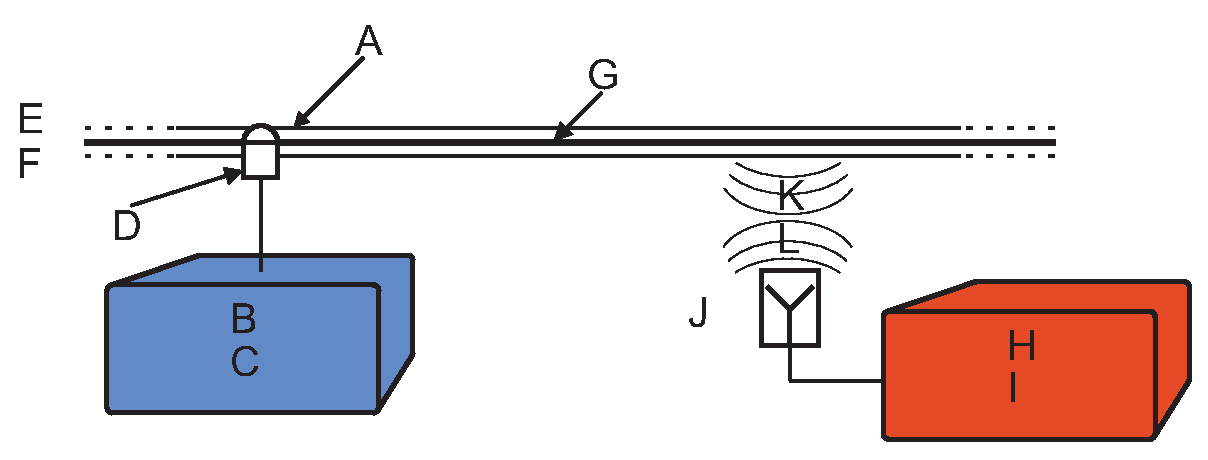
\includegraphics[width=0.49\textwidth]{images/Hybrid_channel.eps}
	\caption{The block diagram of a hybrid PLC-WLC system.}
	\label{Hybchannel}
\end{figure}

It is important to highlight that the symmetry of the hybrid \ac{PLC}-\ac{WLC} channel magnitude response is verified when the transmitter and the receiver have the same access impedance, see \cite{thiago:hyb}. Mathematically, $h_{PW}(t,\tau)=h_{WP}(t,\tau)$ agrees with the results presented in \cite{Galli:indoor}, which focuses only on \ac{PLC} channels. Due to the specific characteristics of each media (e.g., power line and air), the symmetry property does not hold true for the additive noises $V_{PW}(t)$ and $V_{WP}(t)$ \cite{thiago:hyb}. 

Similar to \ac{PLC} systems, the hybrid \ac{PLC}-\ac{WLC} system operates in the baseband. Therefore the deduction adopted earlier is directly applied to the channel impulse responses of the \ac{PLC}-\ac{WLC} channels. As a result, the vectorial representation of the channel frequency magnitude is also denoted by the vector $|{\bf H}|$. 
 
Given the aforementioned formulation, the following research questions arise: \textit{What kind of statistical distributions are suitable for modeling the random variables that constitute the vector $|{\bf H}|$ under the availability of measured data set obtained from a measurement campaign carried out in Brazilian residences? Could we state that $|{\bf H}|$ is a stationary random process?} The following sections try to answer these challenging research questions.

\section{Modeling Methodology}

With the purpose of addressing the research questions exposed in the previous section, an enhanced statistical modeling method is devised through the top-down approach, aiming to obtain the models of \ac{CFR} magnitudes related to \ac{PLC} and hybrid \ac{PLC}-\ac{WLC} channels. Basically, each element of the \ac{r.v.} ${\bf |H|}$ is assumed to be uncorrelated. This is an interesting approach to come up with simple statistical models to employ ${\bf |H|}$ for performing theoretical analysis related to channel capacity, physical layer security, energy harvesting and cooperative communication, among others.

The statistical modeling can be summarized in searching for the statistical distributions offering the best fits to a data set obtained from a measuring campaign (i.e., measured \ac{CFR} estimates). It means that the type of statistical distribution together with its parameters are the modeling information for each element of the \ac{r.v.}  ${\bf |H|}$. In other words, the model is the chosen statistical distribution together with its parameters.

In addition, it is important to come up with the statistical model of $H(f)=|H(f)|\exp(j\arg{\{H(f)\}})$, which is the Fourier transform of the vector $h(t)$, based on the statistical model of the \ac{r.v.} ${\bf X}$. To do so, a technique capable of yielding a suitable interpolation with a reduced number of parameters and without presenting edge effects, such as that ones reported in \cite{Luis:AI} is a very convenient solution. In fact, standard interpolation technique applied to obtain $H(e^{j\omega})$ from the vector $\bf H$ demands a large number of parameters \cite{mitra} because all elements of the vector $\bf H$ are used for the interpolation purpose. Moreover, it is important to point out that  $H(f)=H(j\Omega)|_{\Omega = 2\pi f}$ is easily obtained from $H(e^{j\omega})$ \cite{mitra}. Based on the fact that we are yielding statistical distributions for the elements of the \ac{r.v.} ${\bf X}$, the interpolation technique is applied to the set of parameters of the statistical distribution modeling each element of the \ac{r.v.} ${\bf X}$.

Regarding the chosen statistical distribution, we can assume that $\alpha_u (\omega) = F_u(\omega; \alpha_{1,u}, \cdots, \alpha_{N,u})$, in which $\omega \in [0,2\pi)$, is such that $\alpha_{k,u} = F_u(2\pi k/N); \alpha_{1,u}, \cdots, \alpha_{N,u}),k=0,1,\cdots,N-1$. In this context, the problem of interpolation consists of finding an approximation $P_u(\omega)$ for the function $F_u(\omega)$ within the defined class of functions, in the way that it can obtain the same values at the points $\omega_k = 2\pi k/N$ (i.e., $F_u(\omega_k)=P_u(\omega_k)$). The Lagrange Interpolation is the direct solution to obtain $P_u(\omega)$; however the degree of interpolating Lagrange polynomial is strictly related to the amount of points (nodes)  $\omega_k = 2\pi k/N$, which makes the problems with high number of input data difficult to solve. The use of Splines can mitigate this problem because it divides the interval into $L$ subintervals, constructs the interpolating polynomial $P_{u,l}(\omega),l=1,\cdots,L$ in the $l$-th subinterval separately and groups the resulting interpolation polynomials to obtain $P_u(\omega)$. Another advantage of the Splines is its capacity of avoiding the Runge's phenomenon. In this contribution we apply the cubic Splines \cite{Spline} due to their characteristics of not needing to use uniform intervals of interpolation, producing smoother curves and interpolating the bounds of the intervals, generating a continuous curve over the chosen frequency subband. 

Based on the aforementioned discussion, the proposed method to obtain the statistical model of the \ac{r.v.} $\bf X$ can be organized in four steps. Essentially, the method consists on trying several statistical distributions to model each element of the \ac{r.v.} $\bf X$, choosing the best statistical distribution by adopting well-established criteria and performing the approximation of the function by using an interpolation technique. The following steps implement the proposed method:
\begin{itemize}
	\item \textbf{Step \#1}: Model all elements of the \ac{r.v.} ${\bf X}$ with the set of statistical distributions that addressed the characteristics of its elements. It is important to highlight that ${\bf |H|} \in \mathbb{R}_{+}^{N\times 1}$ and ${\bf \Theta \in \mathbb{R}}_{+}^{N \times 1}|0 \leq { \Theta_k} \leq 2\pi$ determine the usefulness of distinct set of statistical distributions for modeling the two types of components of the \ac{r.v.} ${\bf X}$ (i.e., ${\bf |H|}$ and ${\bf \Theta}$).
	\item \textbf{Step \#2}: Appraise the set of statistical distributions, for each element of the \ac{r.v.} ${\bf X}$ in order to select the best statistical distribution. In this sense, we consider the majority vote rule \cite{vote} over four chosen criteria (\ac{MLE}, \ac{AIC}, \ac{BIC}, and \ac{EDC} information criteria \cite{Dorea:Sim}, \cite{Cabral:Multi}, \cite{Andrei:Meas}). By considering \ac{MLE} criterion, the best statistical modeling is the distribution that achieves the maximum value, whereas for the \ac{AIC}, \ac{BIC}, and \ac{EDC} information criteria, the best modeling is the statistical distribution that achieving minimum values.
	\item \textbf{Step \#3}: Find the statistical distribution yielding the best statistical modeling for the large number of elements of the \ac{r.v.} ${\bf X}$. This statistical distribution is chosen as the statistical distribution for all elements of the \ac{r.v.} ${\bf X}$. The set of parameters (i.e., $\mathcal{C}_{X_k} = \{ \alpha_{k,1}, ...., \alpha_{k,U} \}$ ) associated with the chosen statistical distributions for each element of the \ac{r.v.} $\bf X$ is obtained.
    \item \textbf{Step \#4}: Interpolate the parameters in the previous step using the cubic Spline interpolation approximation for obtaining $\mathcal{C}_f = \{ \alpha_{1}(f), ...., \alpha_{U} (f)\}$. This procedure consists on dividing the obtained values into $L$ subintervals delimited by $\omega_{l,\textnormal{lower}}$ and $\omega_{l,\textnormal{upper}}$ bounds, and evaluating a third-degree polynomial that describes the $l^{th}$ subinterval. This evaluation is performed by mapping the $l^{th}$ subinterval to $[0,1]$ and using the values of evaluated tangents at the upper and lower bounds of the interval. Regarding the frequency band (i.e., $f\in[0,B)$, the coefficients of the $l^{th}$ polynomial are them obtained and can be used to generate a reliable continuous waveforms of the parameters from the chosen statistical distributions in the continuous-time domain.    
\end{itemize}

\section{Numerical Results}

%%%%%%%%%%%%%%%%%%% Adicionar aos resultados numericos!!!
%The following organization for modeling the hybrid \ac{PLC}-\ac{WLC} channels was proposed in \cite{thiago:hyb}:
%
%\begin{itemize}
%	\item \textit{short-path} channel: On this scenario, the \ac{WLC} Transceiver may be randomly positioned within a $2$~m radius circle, centered at the outlet in which the \ac{PLC} Transceiver was connected.
%	
%	\item \textit{long-path} channel: On this scenario, the \ac{WLC} Transceiver was randomly placed into a area defined as a swept circle, having an outer and inner radius of $6$~m and $2$~m, respectively, centered at the outlet in which the \ac{PLC} Transceiver was connected.
%\end{itemize}
%%%%%%%%%%%%%%%%%%%

%The statistical analyses were performed by means of a data set constituted by \ac{CFR} estimates of in-home \ac{PLC} channels, which were acquired during a measurement campaign detailed in \cite{Thiago:Characterization}. Altogether $245$ different combinations of outlets pairs were measured, enabling the acquisition of $148,037$ different \ac{CFR} estimates, with an average of $604$ consecutive \ac{CFR} estimates for each channel configuration. The methodology applied to obtain the \ac{CFR} estimate is the one discussed in \cite{Thiago:FR} and it relies on a measurement setup and the use of an \ac{HS-OFDM} scheme \cite{HSOFDM,Picorone}. The measurement setup covers signal generation and acquisition boards, rugged computers, and coupling devices \cite{Luis:AI}, while the \ac{HS-OFDM} scheme is a kind of sounding technique for estimating \ac{CFR} in the discrete time-domain when the data communication channel is in the baseband. This scheme estimates \ac{CFR} of in-home \ac{PLC} channels by encompassing correction \cite{Gardner:Interpolation}, timing synchronization \cite{Hanzo:OFDMSync}, \ac{CFR} estimation \cite{Thiago:FR}, and enhancement of \ac{CFR} estimates \cite{Cardoso:CEzeropad,Ouzzif:CP}. Finally, after applying the aforementioned techniques, the average of $L_a=10$ consecutive \ac{CFR} estimates is obtained and then stored as a valid \ac{CFR} estimate, this last procedure is applied aiming to reduce the impulsive noise influence on the \ac{CFR} estimates.
%
%As described in Section III, once the best statistical distribution for modeling the valid \ac{CFR} magnitudes and phases are chosen, the parameters defining the statistical distributions are stored and then interpolated with the cubic Spline interpolation technique, generating a continuous curve in the frequency domain. This procedure is performed individually for each parameters of the statistical distribution. In order to apply the interpolation technique based on  the cubic Spline, twenty samples of the \ac{CFR} estimates, which are related to frequencies located in the frequency band $(1.7-100$~MHz) were chosen as bounds, resulting in $L=19$ subintervals to be interpolated by the cubic Splines. The number of bounds and their non-uniform spacing were heuristically chosen because the variation of the parameters is distinct within the the frequency band of interest. 

%It is important to emphasize that one \ac{CFR} estimate is obtained during a time interval corresponding to one \ac{HS-OFDM} symbol period $(T_{sym})$ duration and, as a consequence, it assumes that the time interval duration of the \ac{HS-OFDM} symbol must be shorter than the coherence time of the \ac{PLC} channel. Based on the set of parameters of the estimation technique, an enhanced channel estimate is obtained every $T_{sym}=(2N + L_{cp}) T_s = 23.04$~$\mu$s, where $N=2048$ is the number of \ac{BPSK} modulated subcarriers of the \ac{HS-OFDM} symbol, $L_{cp}=512$~samples is the length of the so-called \ac{CP}, $f_s=200$~MHz is the sampling rate and $T_s=1/f_s=5$~ns is the sampling period. According to \cite{Canete:AIPLC}, $600~\mu$s is the minimum time period within which the in-home \ac{PLC} channel can be considered time invariant in Spain, while \cite{Thiago:Characterization} pointed out $950~\mu$s for the Brazilian in-home \ac{PLC} channels. Regardless of the place, the time interval duration of each \ac{CFR} estimation ($T_{sym}$) complies with the coherence time and, as a consequence, we can take it as an advantage to reduce the noise impulsiveness influence on the \ac{CFR} estimates by taking the average of $L_a$ consecutive \ac{CFR} estimates within the coherence time. Moreover, the assumed value of $N$ and the chosen frequency band ($1.7-100$)~MHz, results in \ac{CFR} estimates with a corresponding frequency resolution of $\Delta f=48.83$~kHz, which is shorter than the coherence bandwidth of Brazilian and Spanish in-home PLC channels \cite{Canete:AIPLC,Thiago:Characterization}. Being shorter than the coherence bandwidth means that each sample of  the magnitude of the valid \ac{CFR} estimates is representative for carrying out the statistical analyses. 
%
%In order to perform the statistical analyses of the valid \ac{CFR} magnitudes, the following statistical distributions were adopted: Beta, Birnbaum-Saunders, Gamma, Logistic, Log-normal, Normal, Rayleigh, Rician, t Location-Scale, and Uniform. These statistical distributions cover the well-established ones in the telecommunication field and those applied to model a random variable belonging to $\mathbb{R}_+$. Regarding the valid \ac{CFR} phase, the Beta, Logistic, Normal, t Location-Scale and Uniform distributions were considered. Furthermore, for sake of clearness, all numerical results are presented in the continuous-time domain rather than the discrete-time one. 
%
%Fig. \ref{respfreq} shows $5$ valid estimates of the \ac{CFR} magnitude, considering the aforementioned frequency band. Each valid \ac{CFR} estimate was obtained by averaging  $L_a$ consecutive \ac{CFR} estimates of a \ac{PLC} channel associated with an in-home electric power circuit, which was measured during the measurement campaign. Note that the channel attenuation ranges from approximately $-30$~dB up to $0$~dB. These plots show that the in-home \ac{PLC} channels present a small time-varying behavior during a time interval shorter than $1$~ms once each valid \ac{CFR} estimate covers a time interval equal to $\Delta T = L_a T_{sym} \approx 230.4\mu$s and, as a consequence, $5\Delta T = 1.15$ms. In other words, the coherence time in an in-home Brazilian PLC channel is larger than in Europe and US, as well-reported in \cite{Thiago:Characterization}.
%
%\begin{figure}[h]
%	\centering
%	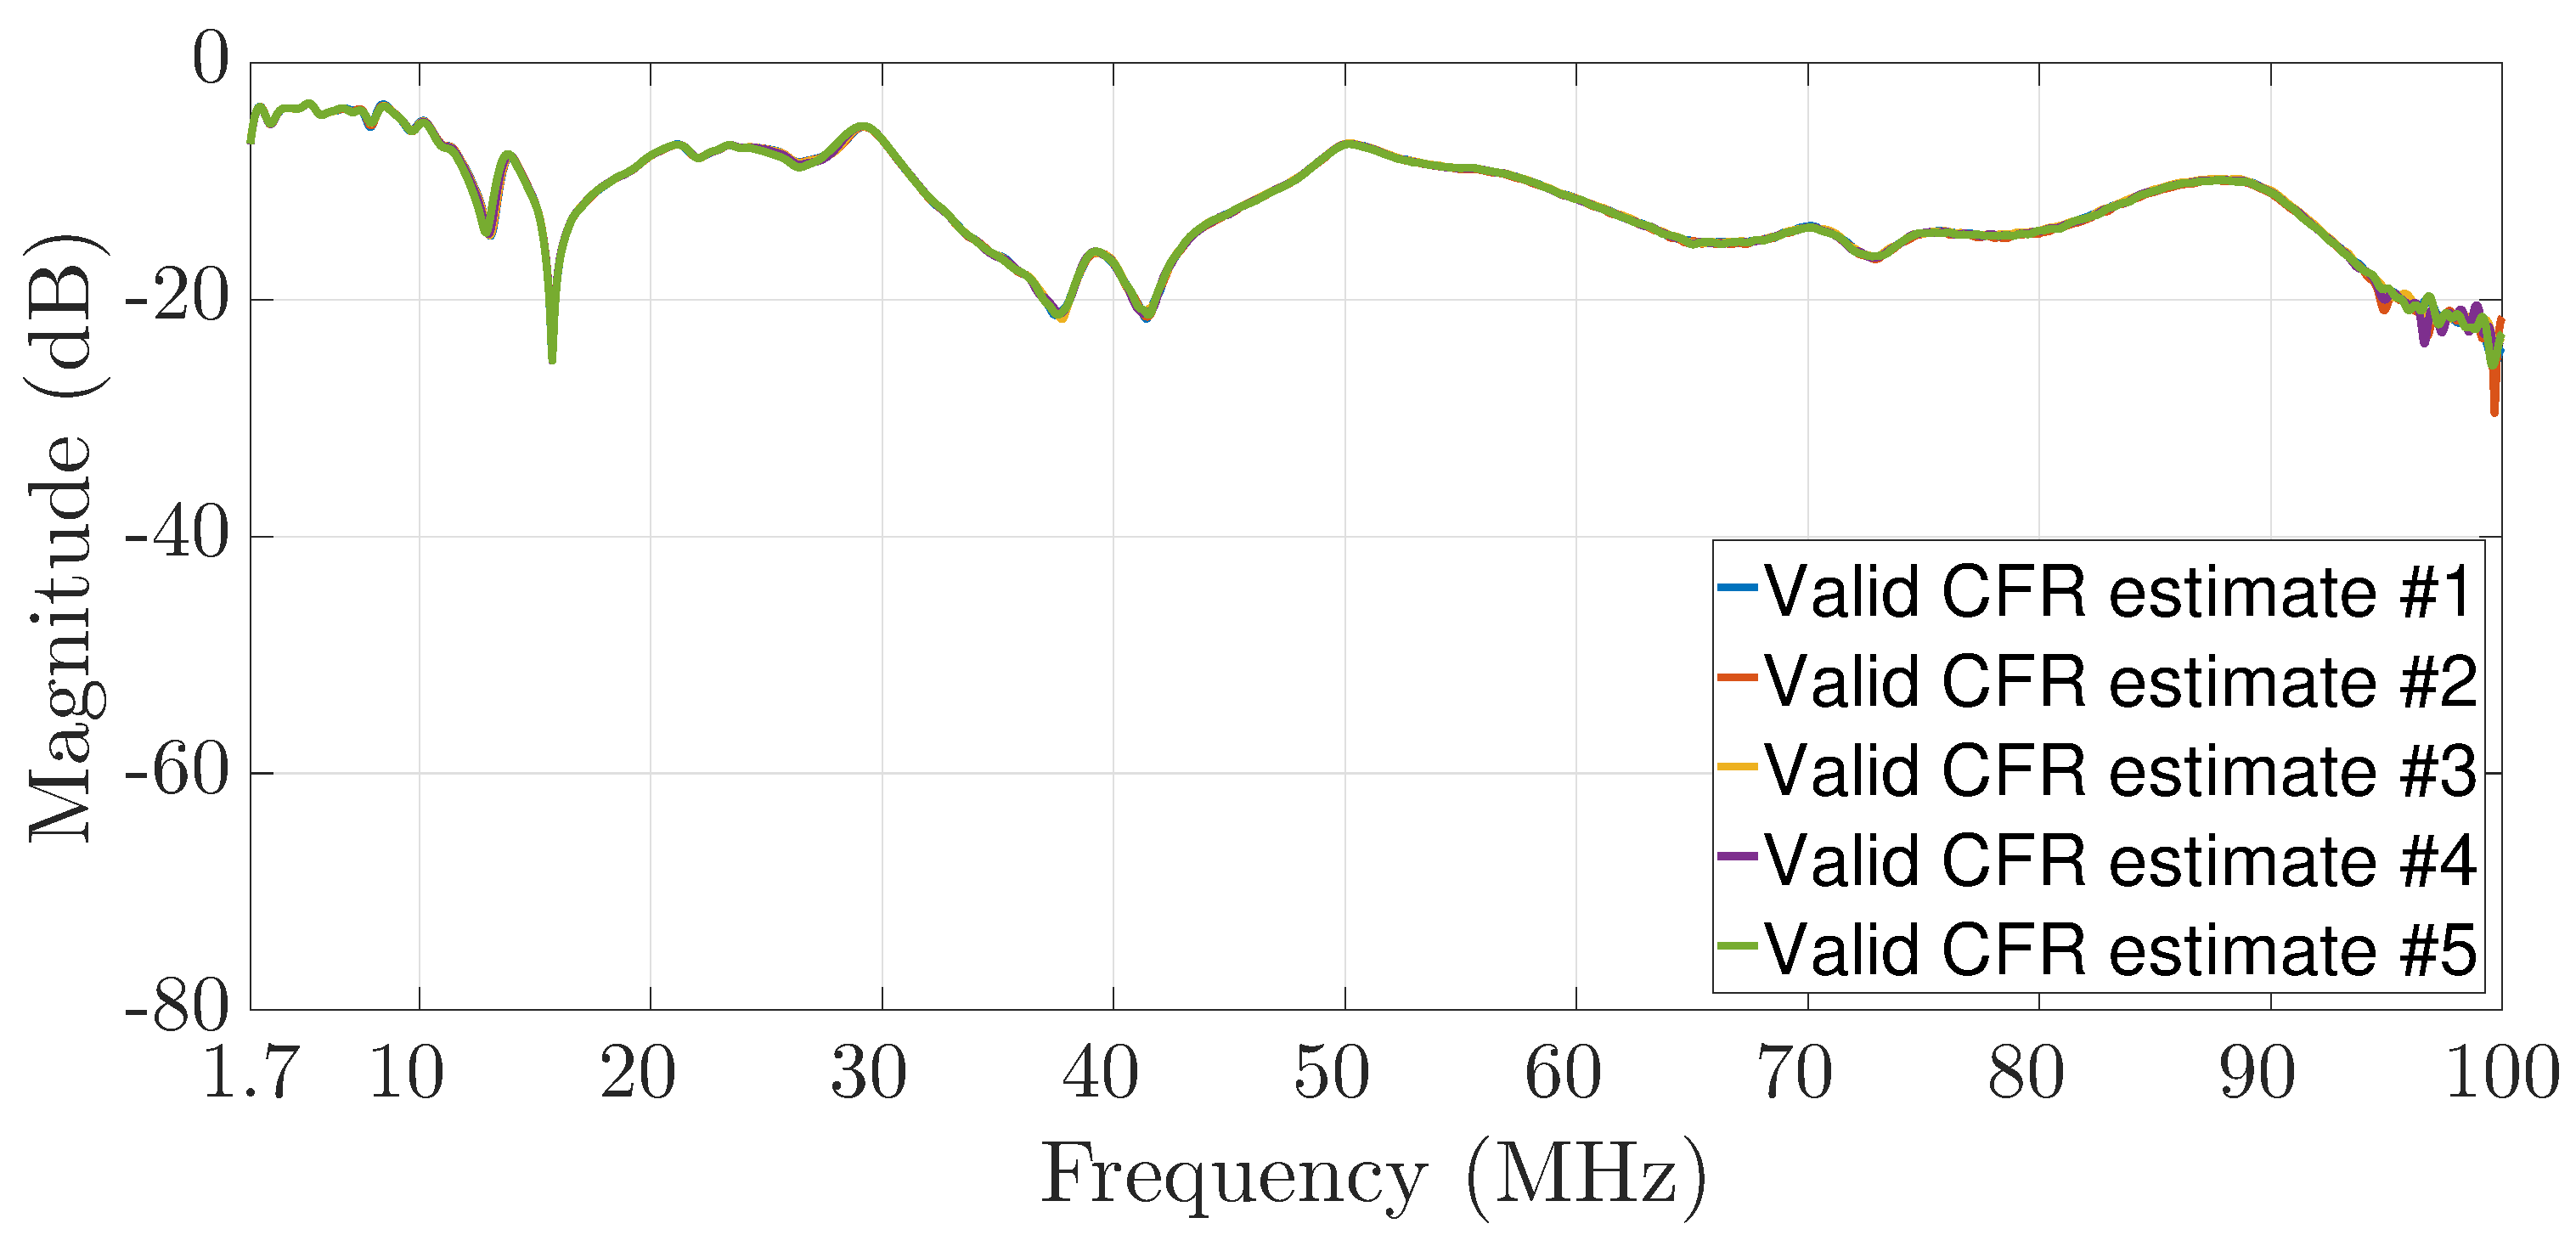
\includegraphics[width=0.49\textwidth]{images/respfreq_1.7.eps}
%	\caption{Five consecutive and valid \ac{CFR} Magnitudes of the measured in-home \ac{PLC} channel.}
%	\label{respfreq}
%\end{figure}
%
%Fig. \ref{MAG_percent} shows the relative frequency of statistical distributions that had modeled, in accord with the adopted criteria, the magnitude of the whole set of valid \ac{CFR} estimates. It is noted that there is not only a single distribution that models the majority of the magnitudes, but three different statistical distributions that stand out as possible candidates to model the \ac{CFR} magnitudes. As a matter of fact, in 35\% of the \ac{CFR} estimates data set the Beta distribution resulted in the best model, in 30\% of it  the Birnbaum-Saunders distribution offered the best modeling and in 24\% of it the Log-normal distribution yielded the best modeling. 
%
%\begin{figure}[h!]
%	\centering
%	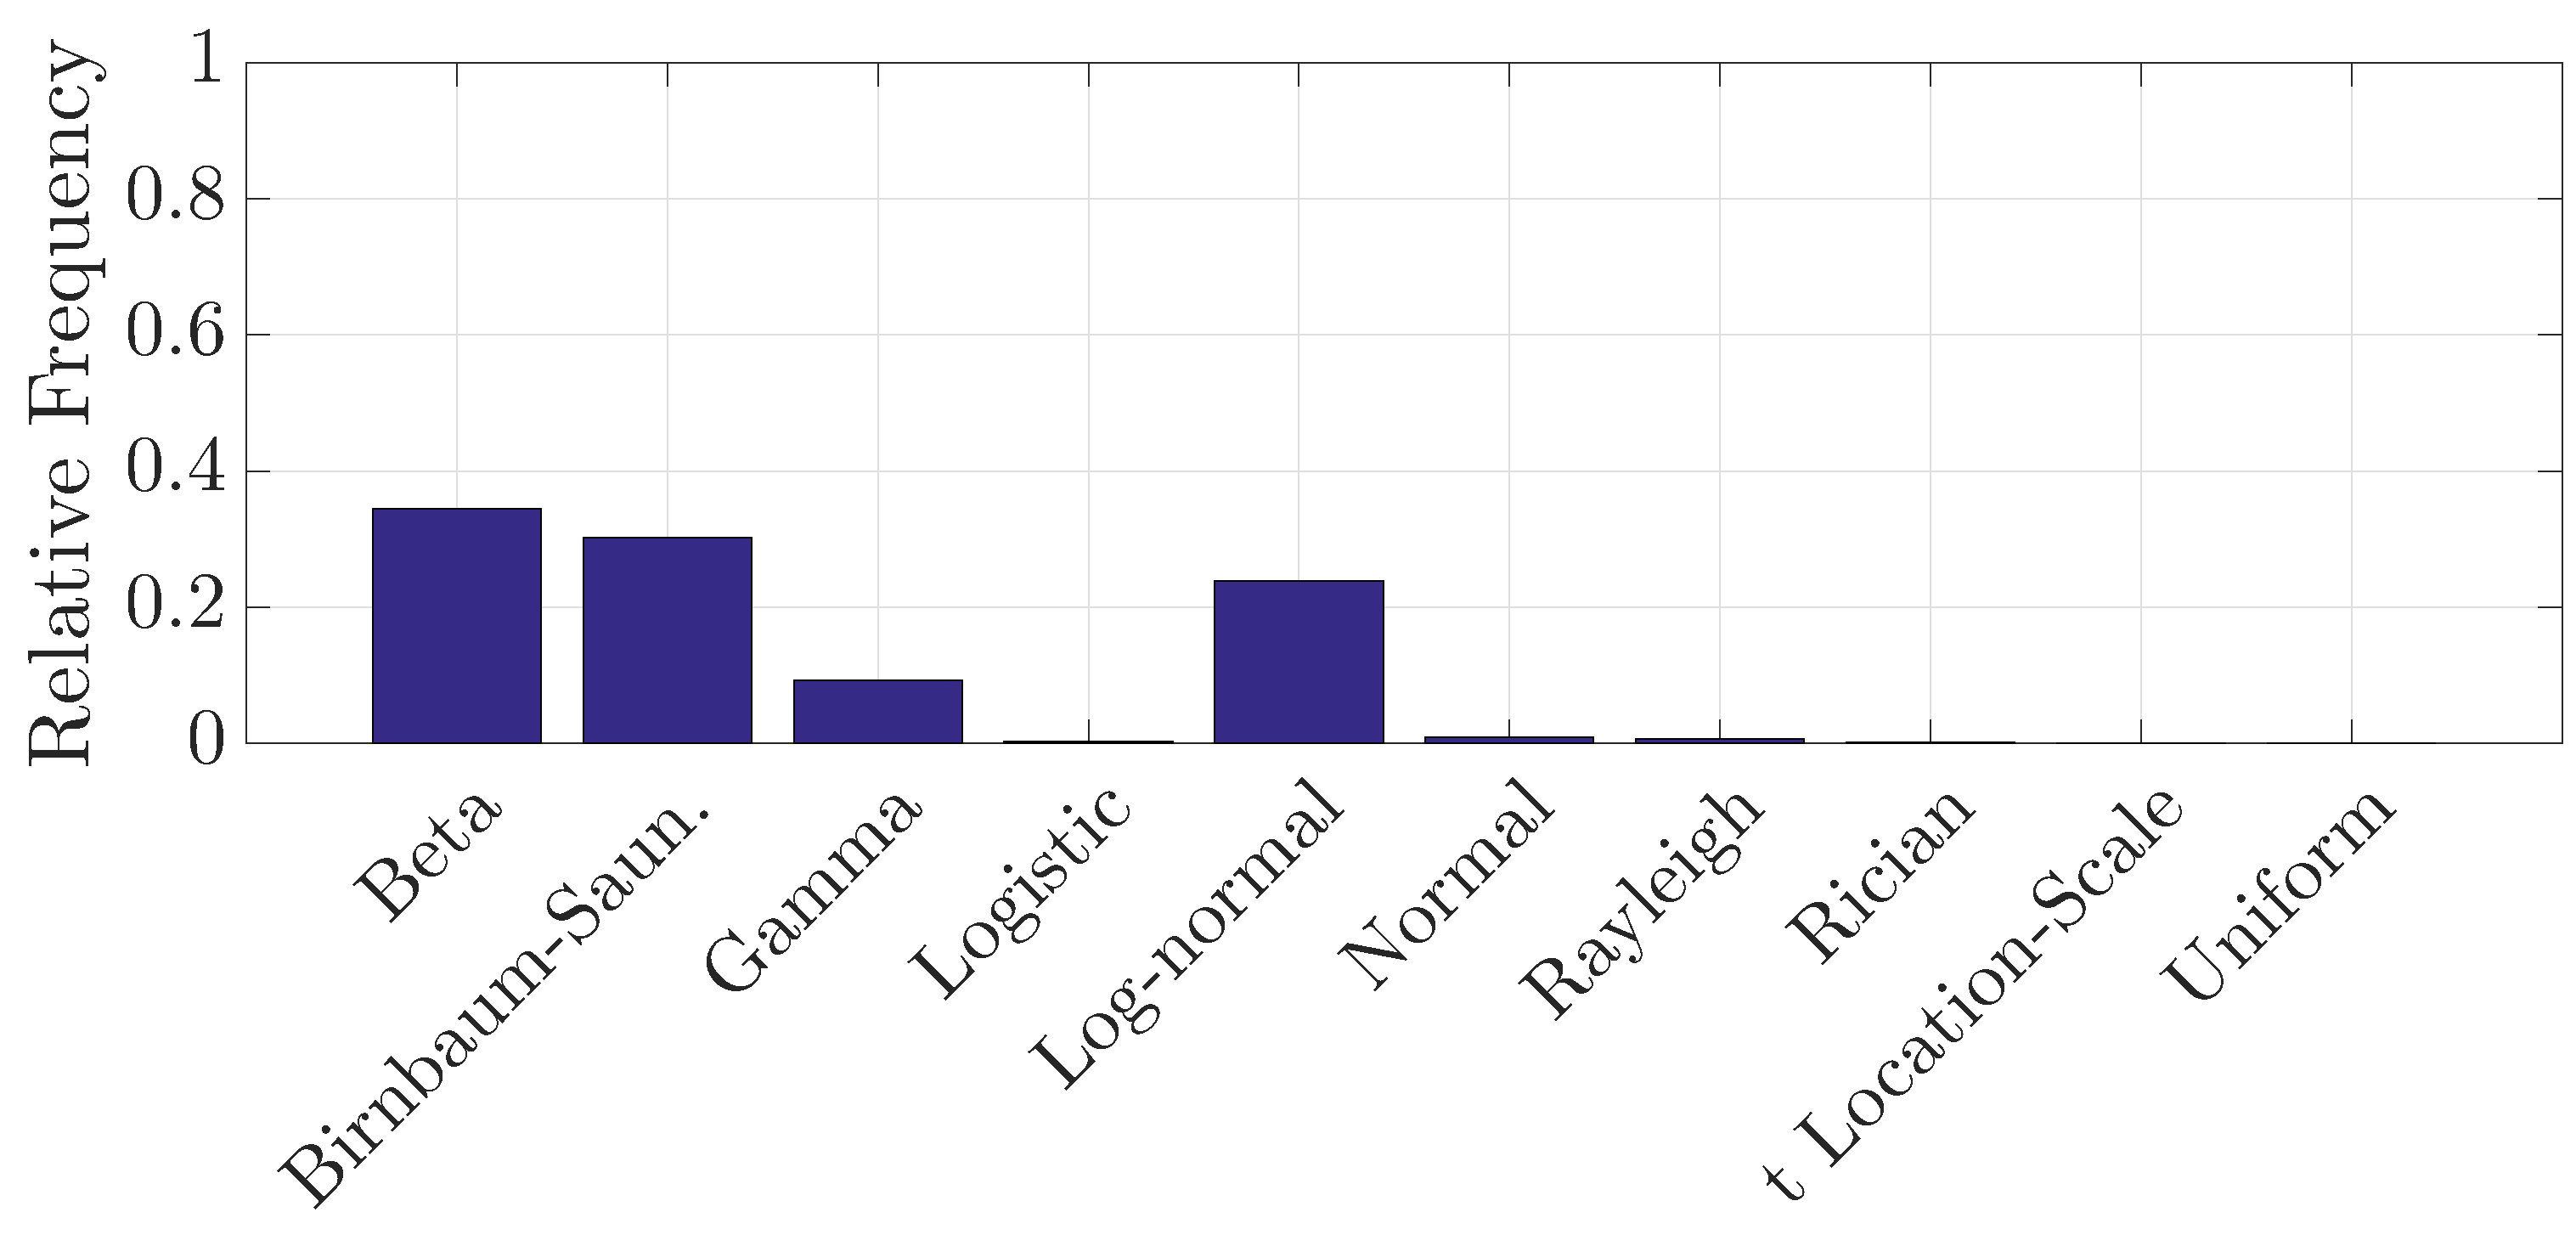
\includegraphics[width=0.49\textwidth]{images/Mag_percent.eps}
%	\caption{The relative frequency associated with the chosen statistical distribution that best models the \ac{CFR} magnitude in accord with the adopted criteria.}
%	\label{MAG_percent}
%\end{figure}
%
%In order to evaluate which of the three distributions is the best choice to model the magnitude component of the \ac{CFR} estimates, we define the log-likelihood ratio as
%\begin{equation}
%	\rho_{LLE} (f) \triangleq \dfrac{LLE(\mathcal{A},f )}{\max_{\mathcal{A}} LLE(\mathcal{A},f)},
%\end{equation}
%where $ LLE(\mathcal{A})$ is the value of the log-likelihood associated with the statistical distribution denoted by $\mathcal{A}\in\{${Beta, Birnbaum–Saunders, Gamma, Logistic, Log-normal, Normal, Rayleigh, Rician, t Location-Scale, Uniform}$\}$ and $\max_{\mathcal{A}} LLE(\mathcal{A})$ is the value of the log-likelihood related to the statistical distribution yielding the best modeling. Note that the best results are achieved when $\rho_{LLE} (f) \rightarrow 1.0$. Fig. \ref{fig:Log_like} shows the values of  $\rho_{LLE}(f)$ for the three best statistical distributions candidates to model the magnitude of the valid \ac{CFR} estimates. Note that the vertical axis was limited to the range from $0$ up to $5.0$ to facilitate the visualization and the comparison among the log-likelihood ratio ($\rho_{LLE} (f)$) curves. These curves emphasize the suitability of the Beta distribution to model the samples of the magnitude of the valid \ac{CFR} estimates. Overall, the results presented in Fig. \ref{MAG_percent} and Fig. \ref{fig:Log_like} strongly indicate the use of the Beta distribution to model the magnitude of the valid \ac{CFR} estimates of the measured in-home Brazilian \ac{PLC} channels. This result is different from previous works that had suggested the Log-normal or Rayleigh distributions to model this magnitude, see \cite{Galli:Wireline,RayleighPLC}.
%
%\begin{figure}[h!]
%	\centering
%	\psfrag{AAA}[c][c][1]{$\rho_{LLE} (f)$}
%	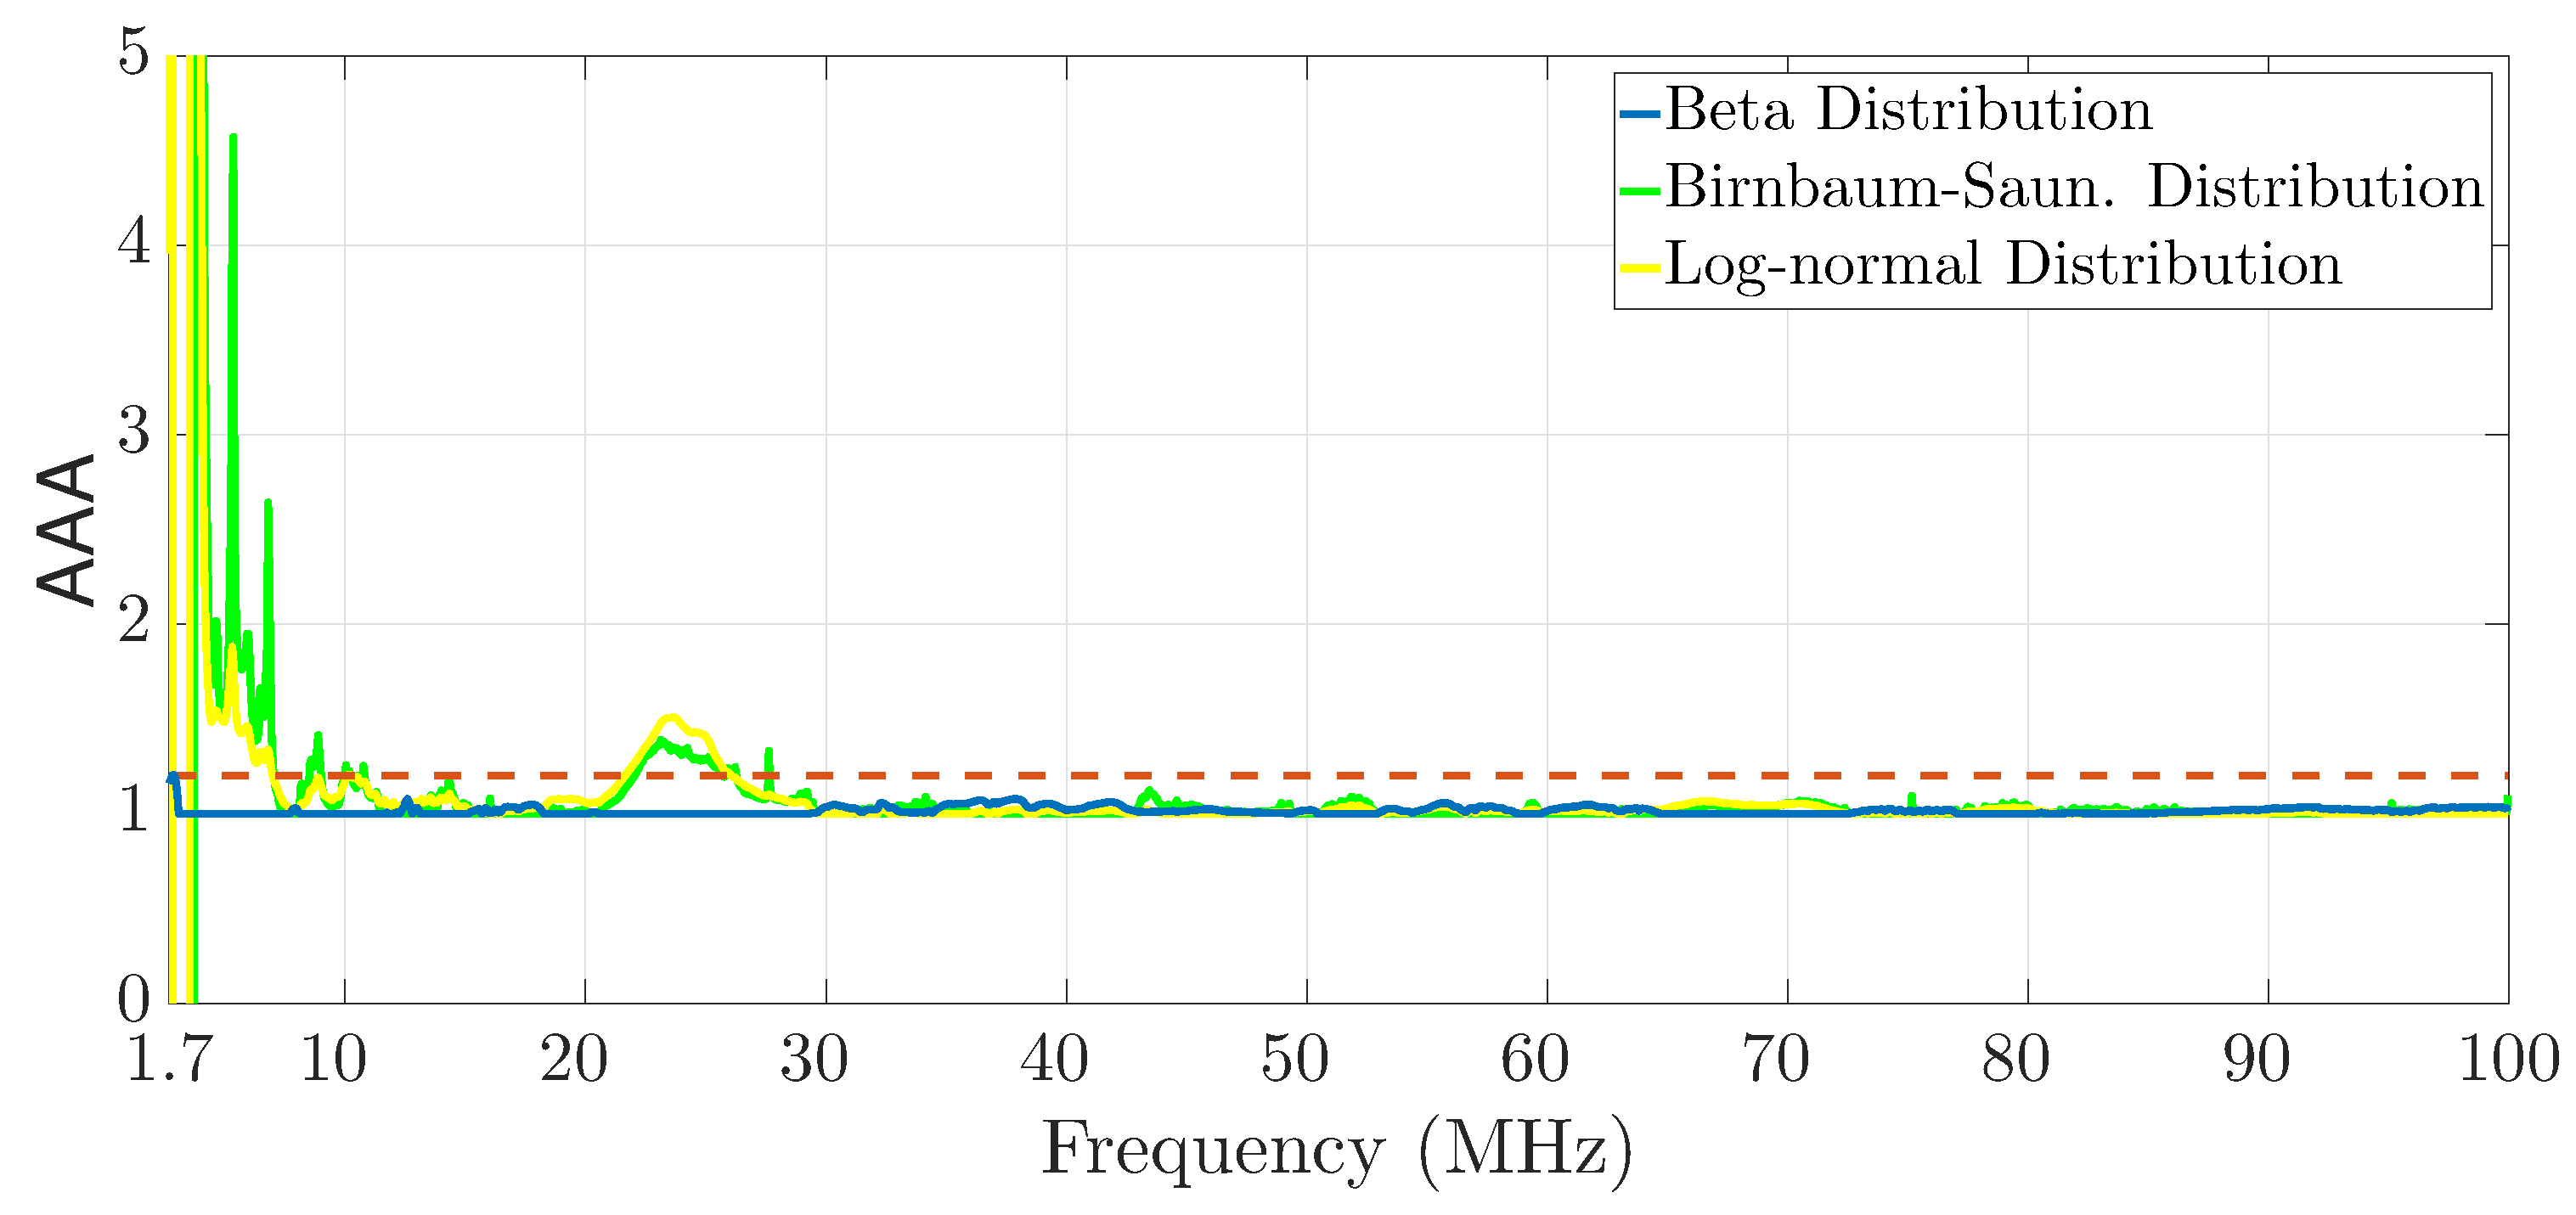
\includegraphics[width=0.5\textwidth]{images/LLH_BETA_BIRN_LogN_1.7.eps}
%	\caption{The log-likelihood ratio for the the following statistical distributions: Beta, Birnbaun-Saunders, and Log-normal.}
%	\label{fig:Log_like}
%\end{figure}
%
%Based on the aforementioned discussion, we can model the magnitude of the valid \ac{CFR} estimates by using only one statistical distribution (i.e., the Beta distribution). However, the statistical analysis of the magnitude of the valid \ac{CFR} estimates shows that each sample of it must be modeled with a set of parameters of the Beta distribution assuming different values. If $\mathcal{C}_{|H_k|} = \{\alpha_{k,1},\alpha_{k,2}\}$, where $k=0,1,\cdots,N-1$,  $\alpha_{k,1} = \alpha[k]$ and $\alpha_{k,2} = \beta[k]$, are the two parameters ($U=2$) of the Beta distribution associated with the $k$-th sample of the magnitude of a valid \ac{CFR} estimate, then Fig. \ref{mag_example} and Fig. \ref{mag_example2} show the statistical models for two different values of frequency: $f=52.1$~MHz ($f = 1067\Delta f$) and $f=78.1$~MHz ($f = 1600\Delta f$), respectively. The parameters of the Beta distribution are  $\alpha(1067 \Delta f) = \alpha_{1067,1}=0.717$ and $\beta( 1067 \Delta f) = \alpha_{1067,2} = 10.435$; $\alpha(1600 \Delta f) = \alpha_{1600,1} = 0.780$ and $\beta( 1600 \Delta f) = \alpha_{1600,2}=17.772$ for $f=52.1$~MHz and $f=78.1$~MHz, respectively.
%
%\begin{figure}[h!]
%	\centering
%	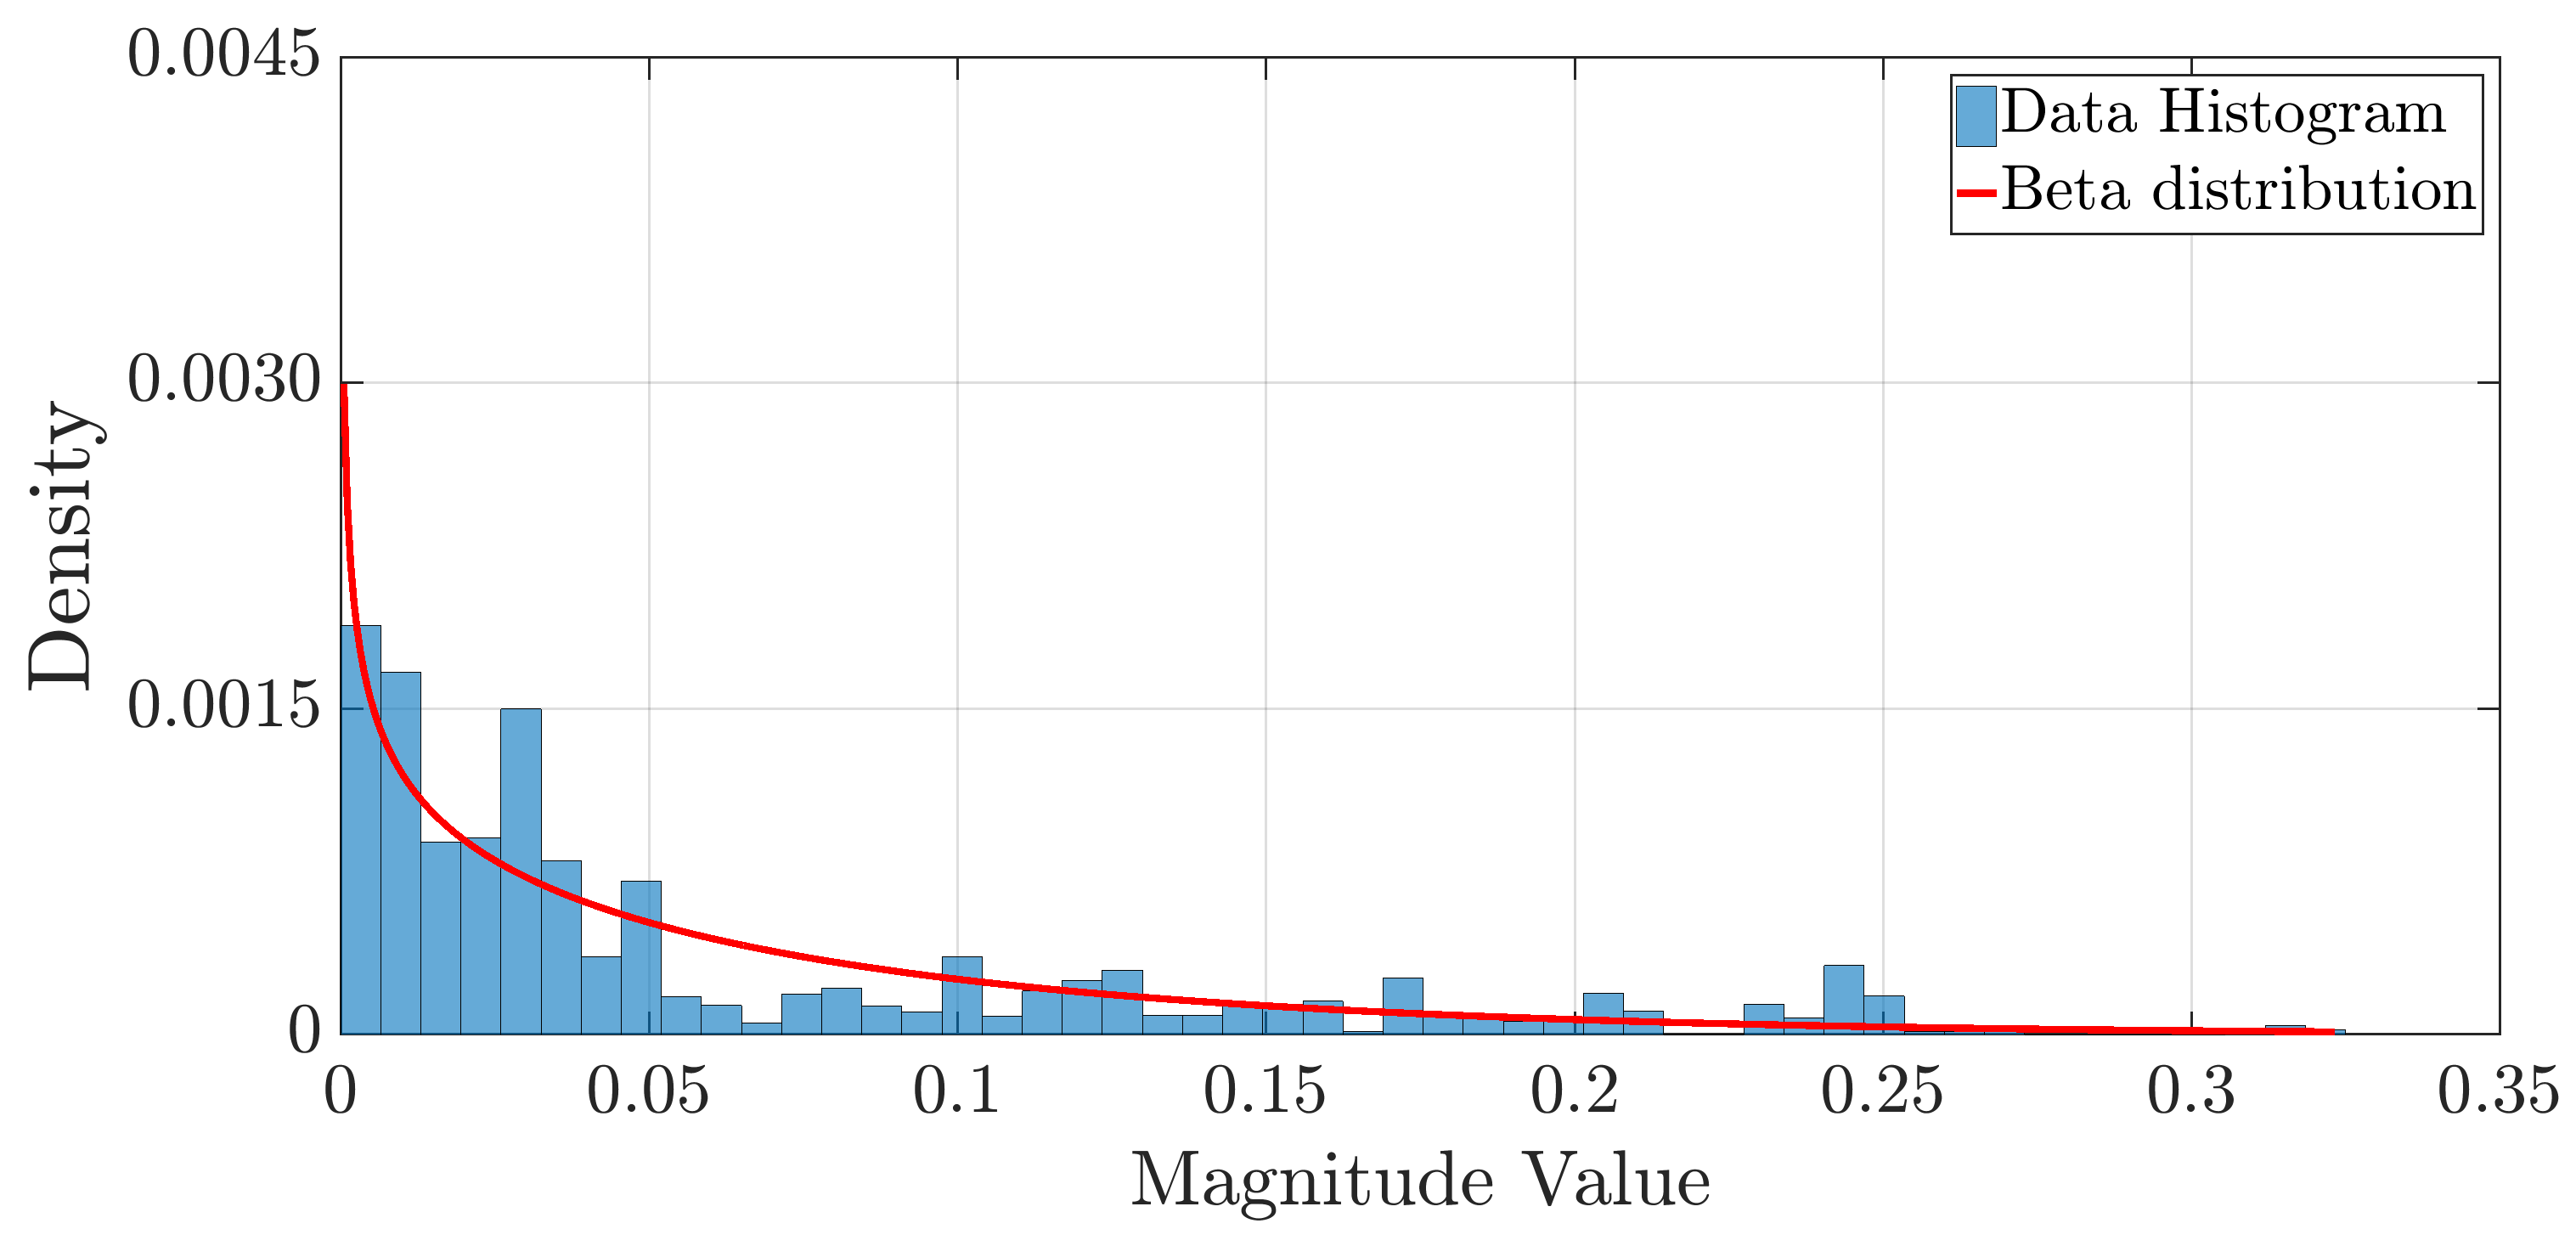
\includegraphics[width=0.49\textwidth]{images/Mag_hist_2.eps}
%	\caption{The relative frequency of the magnitude of the valid \ac{CFR} estimates at the sample $k = 1067$ ($k\Delta f= 52.1$~MHz) and the modeling based on the Beta distribution.}
%	\label{mag_example}
%\end{figure}
%
%\begin{figure}[h!]
%	\centering
%	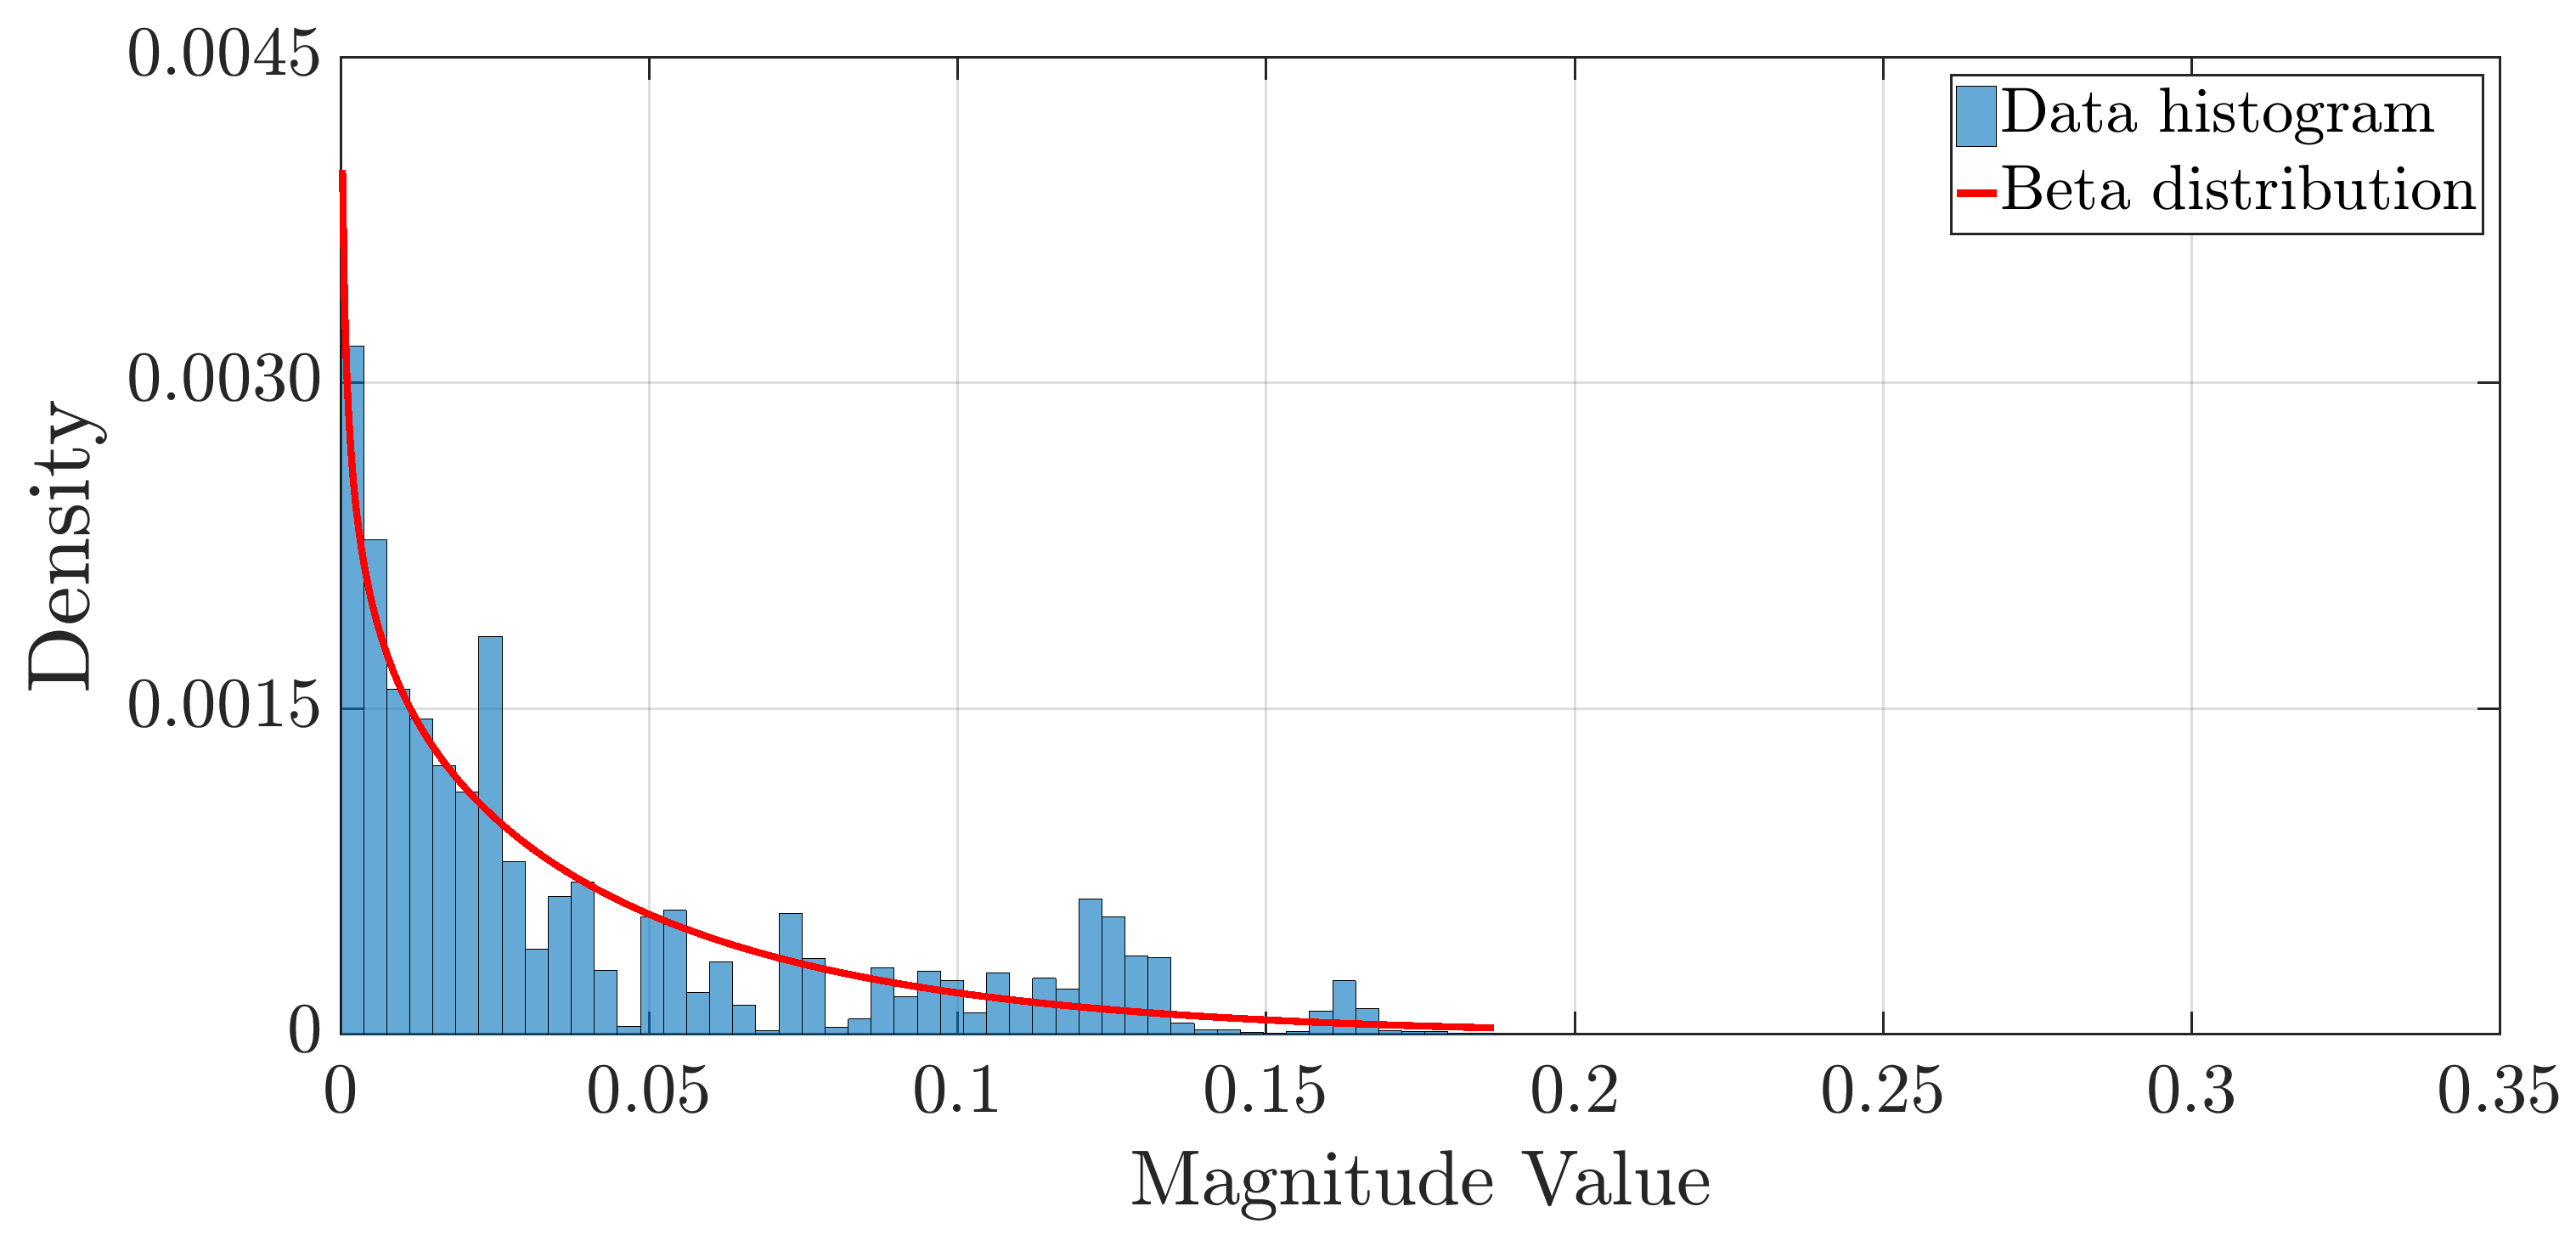
\includegraphics[width=0.49\textwidth]{images/Mag_hist2_2.eps}
%	\caption{The relative frequency of the magnitude of the valid \ac{CFR} estimates at the sample $k = 1600$ ($k\Delta f= 78.1$~MHz) and the modeling based on the Beta distribution.}
%	\label{mag_example2}
%\end{figure}
%
%By interpolating the parameters values $\alpha(k\Delta f)$ and $\beta(k\Delta f)$ of the Beta distributions associated with each sampled valid \ac{CFR} estimates and by using the method implemented in Algorithm \ref{Algo2}, we obtain the continuous curves of parameters $\alpha(f)$ and $\beta(f)$, over the desired frequency band $(1.7-100$~MHz). Figs. \ref{Fit_alfa} and \ref{Fit_beta} shows these curves for the parameters $\alpha(f)$ and $\beta(f)$ after the cubic Spline interpolation process is applied on the $L=19$ subintervals. Furthermore, Table \ref{table_alfa} lists the cubic Spline coefficients for modeling the parameter $\alpha(f)$, of the valid \ac{CFR} magnitude. Similarly, Table \ref{table_beta} lists the cubic Spline coefficients for modeling the parameter $\beta(f)$. As a result, the coefficients values, the waveforms  $\alpha(f)$ and $\beta(f)$, and the Beta distribution define the random process representing the magnitude of the valid \ac{CFR} estimates, named $|{\bf H}|$, in the continuous-time domain.
%
%\begin{figure}[h]
%	\centering
%	\psfrag{Interval Boundsaa}[c][c][0.75]{Interval Bounds}
%	\psfrag{AAA}[c][c][0.75]{~~~~~~$\alpha(k \Delta f)$}
%	\psfrag{BBB}[c][c][0.75]{~~$\hat{\alpha}(f)$}
%	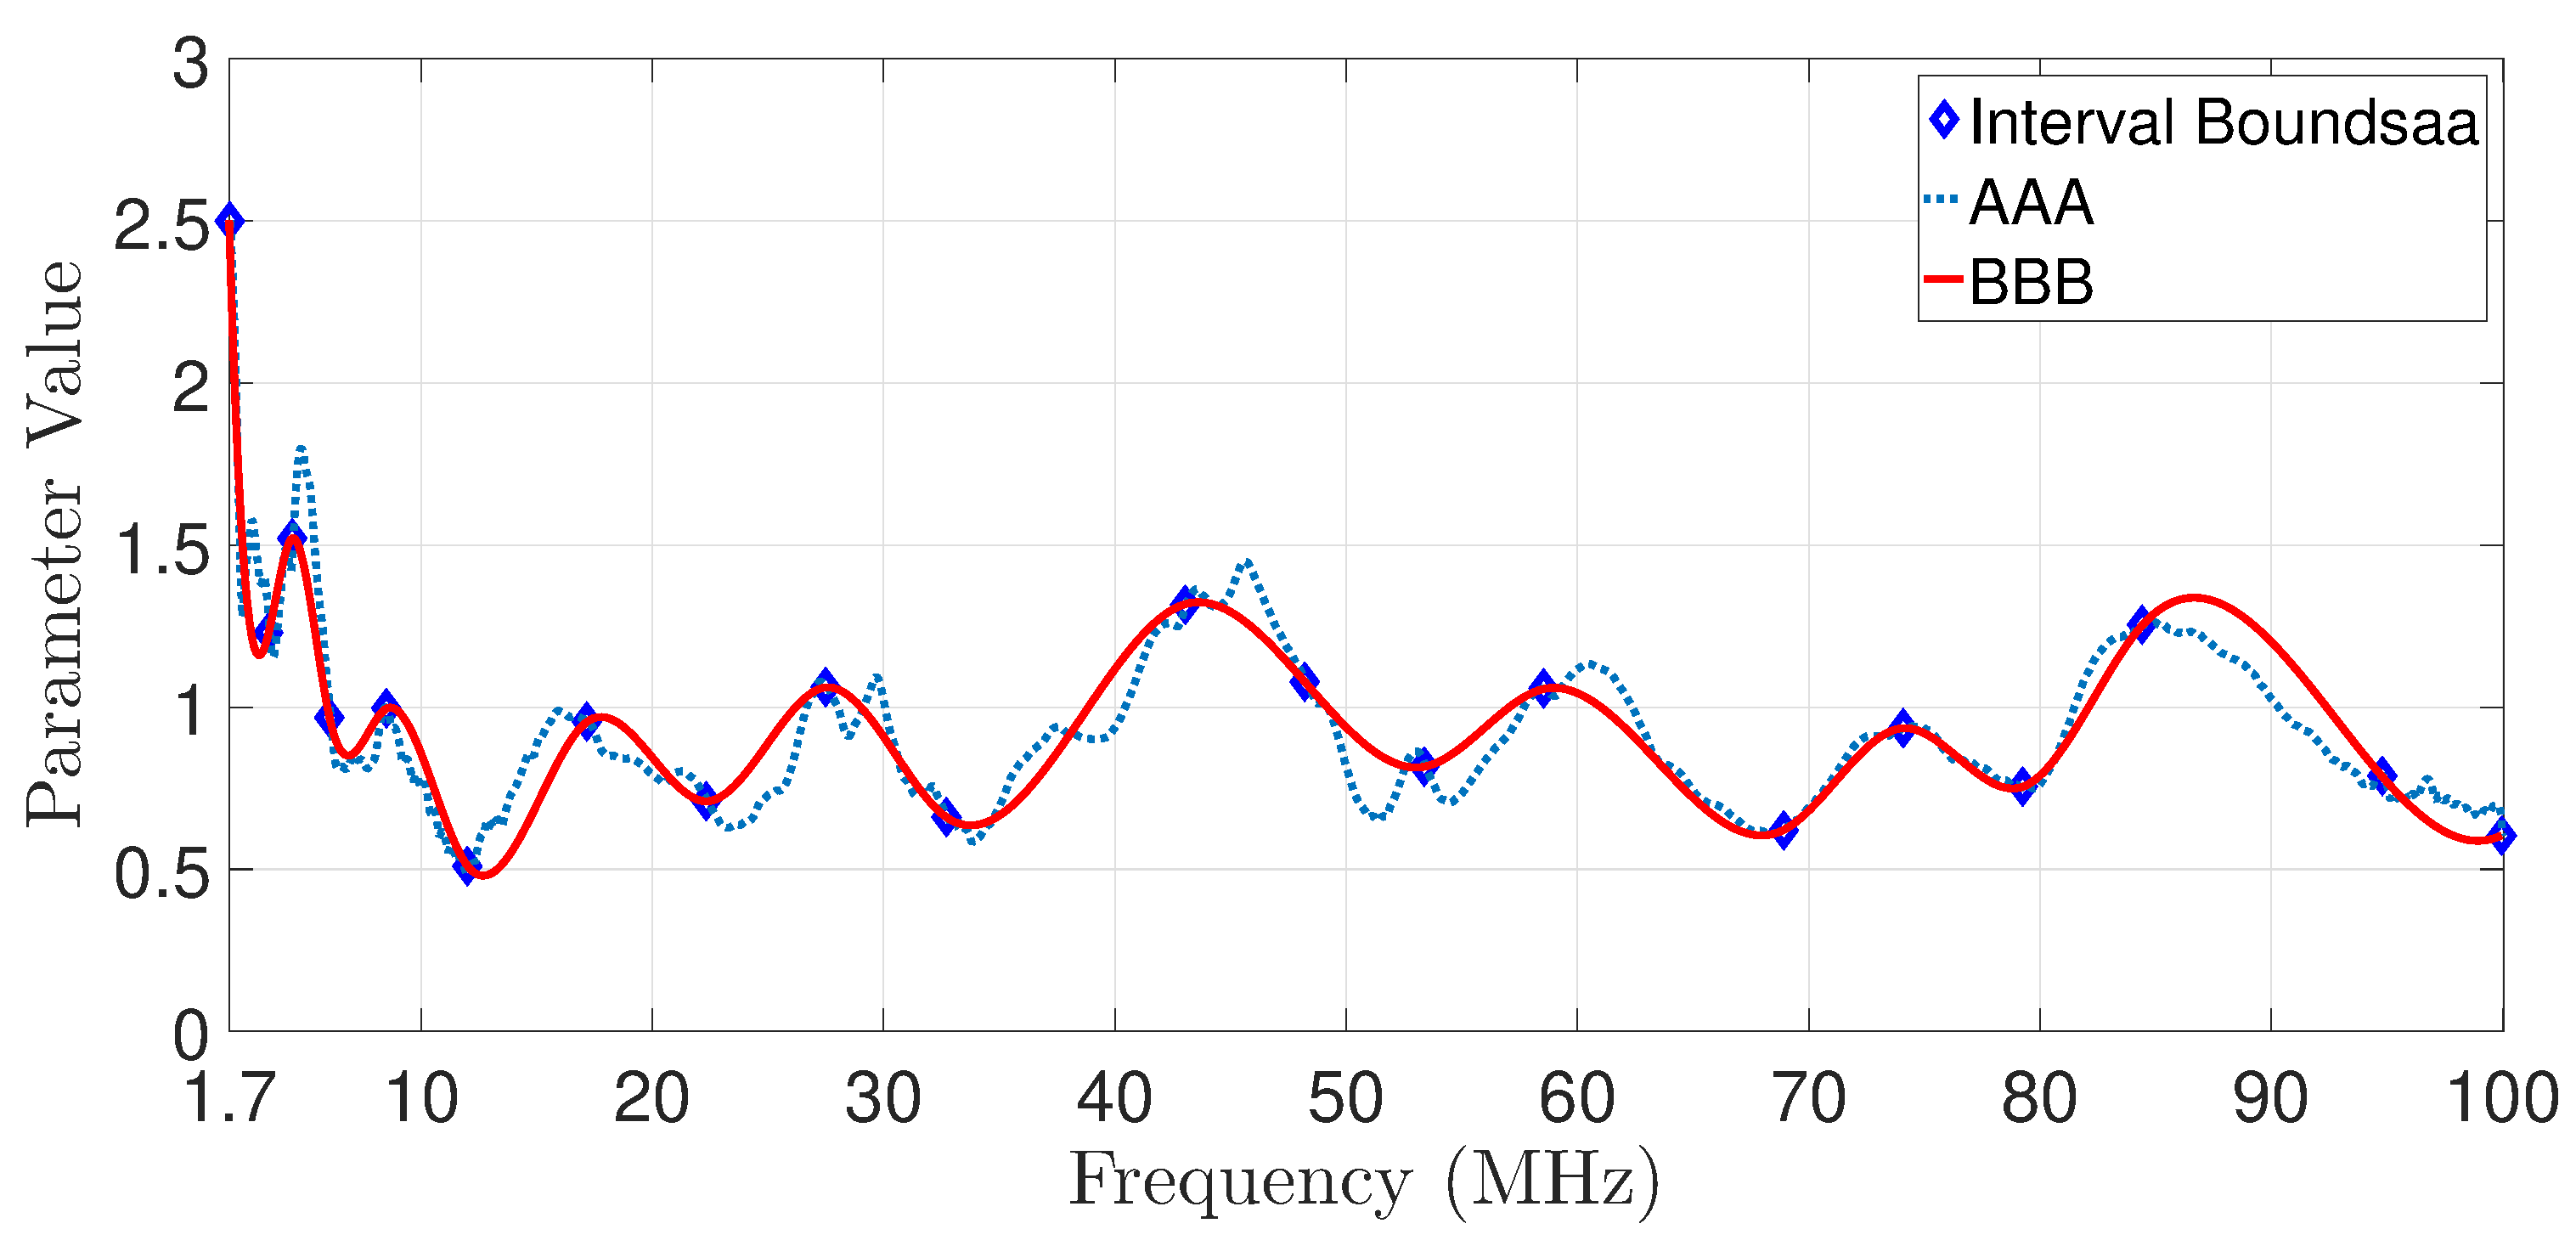
\includegraphics[width=0.49\textwidth]{images/Alfa_fit_1.7.eps}
%	\caption{The result of the interpolation technique based on cubic Splines applied to obtain $\alpha(f) = \zeta_1(f)$ for the Beta distribution ($\alpha(k \Delta f)$ are the original values of the parameter and $\hat{\alpha}(f)$ is the interpolated curve).}
%	\label{Fit_alfa}
%\end{figure}
%%The result of the interpolation technique based on cubic Splines applied to obtain $\alpha(f)=\alpha_1(f)$ for the Beta distribution.
%
%\begin{figure}[h]
%	\centering
%	\psfrag{Interval Boundsaa}[c][c][0.75]{Interval Bounds}
%	\psfrag{AAA}[c][c][0.75]{~~~~~~$\beta(k \Delta f)$}
%	\psfrag{BBB}[c][c][0.75]{~~$\hat{\beta}(f)$}
%	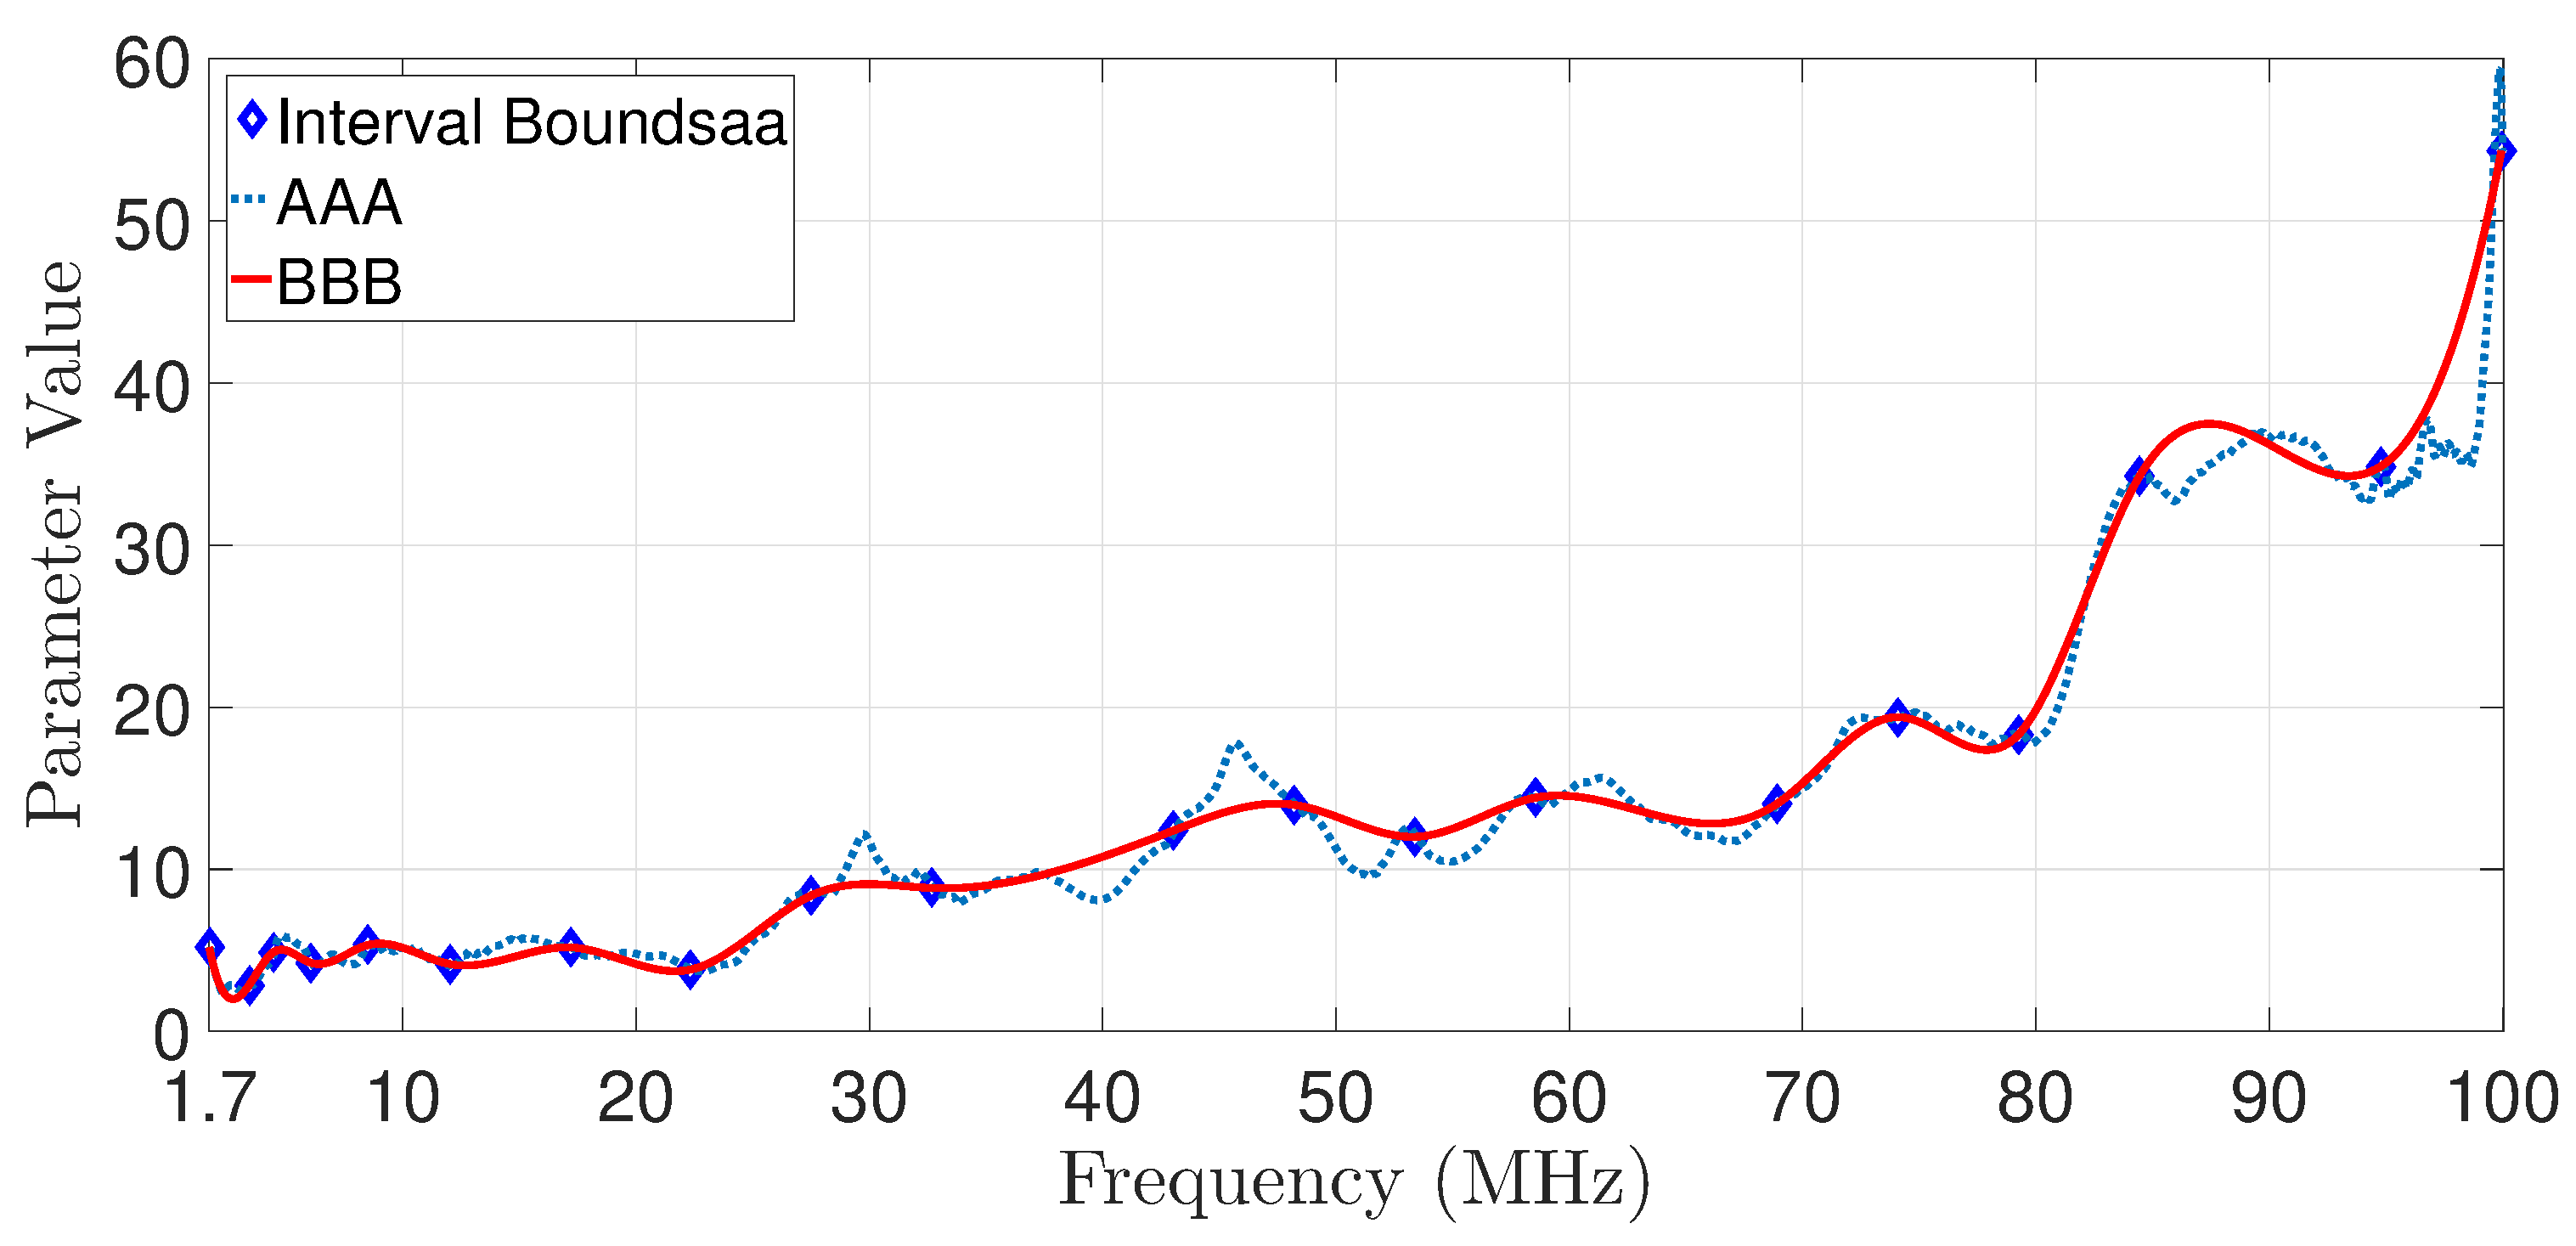
\includegraphics[width=0.49\textwidth]{images/Beta_fit_1.7.eps}
%	\caption{The result of the interpolation technique based on cubic Splines applied to obtain $\beta(f) = \zeta_2(f)$ for the Beta distribution ($\beta(k \Delta f)$ are the original values of the parameter and $\hat{\beta}(f)$ is the interpolated curve).}
%	\label{Fit_beta}
%\end{figure}
%%The result of the interpolation technique based on cubic Splines applied to obtain $\beta(f)=\alpha_2(f)$ for the Beta distribution.
%
%\begin{table*}[h]
%	\setlength\extrarowheight{4.5pt}
%	\centering
%	\caption{$\alpha(f)$ parameter: Coefficients of the cubic Splines for the $L=19$ subintervals.}
%	\label{table_alfa}
%	\begin{tabular}{|C{4cm}|C{3cm}|C{3cm}|C{3cm}|C{3cm}|m{0cm}}
%		\cline{1-5}
%		Frequency Band (MHz)           		   & $a_u$    			  & $b_u$      			 & $c_u$   		 		& $d_u$&\\ \cline{1-5}
%		$1.70\textless \mid f\mid \leq 3.42$   & -2.6528 $\times 10^{-5}$ & 0.0033  				 & -0.1197 					& 2.5007 &\\ \cline{1-5}
%		$3.42\textless \mid f\mid \leq 4.44$   & -2.6528 $\times 10^{-5}$ & 5.2561 $\times 10^{-4}$  & 0.0146  					& 1.2292 &\\ \cline{1-5}
%		$4.44\textless \mid f\mid \leq 6.05$   & 1.7869  $\times 10^{-5}$ & -0.0011                  & 0.0015                   & 1.5211 &\\ \cline{1-5}
%		$6.05\textless \mid f\mid \leq 8.50$   & -5.9605 $\times 10^{-6}$ & 6.2337 $\times 10^{-4}$  & -0.0157                  & 0.9666 &\\ \cline{1-5}
%		$8.50\textless \mid f\mid \leq 12.01$  & 2.0887  $\times 10^{-6}$ & -2.7071 $\times 10^{-4}$ & 0.0019 					& 0.9954 &\\ \cline{1-5}
%		$12.01\textless \mid f\mid \leq 17.19$ & -9.2474 $\times 10^{-7}$ & 1.8046 $\times 10^{-4}$  & -0.0046 					& 0.5114 &\\ \cline{1-5}
%		$17.19\textless \mid f\mid \leq 22.36$ & 6.4104  $\times 10^{-7}$ & -1.1361 $\times 10^{-4}$ & 0.0025  					& 0.9547 &\\ \cline{1-5}
%		$22.36\textless \mid f\mid \leq 27.53$ & -5.6131 $\times 10^{-7}$ & 9.0243 $\times 10^{-5}$  & 5.3515 $\times 10^{-5}$  & 0.7099 &\\ \cline{1-5}
%		$27.53\textless \mid f\mid \leq 32.71$ & 4.7371  $\times 10^{-7}$ & -8.8254 $\times 10^{-5}$ & -2.6432 $\times 10^{-4}$ & 1.0610 &\\ \cline{1-5}
%		$32.71\textless \mid f\mid \leq 43.06$ & -1.7026 $\times 10^{-7}$ & 6.2385 $\times 10^{-5}$  & -0.0025 					& 0.6616 &\\ \cline{1-5}
%		$43.06\textless \mid f\mid \leq 48.24$ & 1.4089  $\times 10^{-7}$ & -4.5902 $\times 10^{-5}$ & 0.0010  					& 1.3178 &\\ \cline{1-5}
%		$48.24\textless \mid f\mid \leq 53.42$ & 1.4415  $\times 10^{-7}$ & -1.0984 $\times 10^{-6}$ & -0.0040 					& 1.0777 &\\ \cline{1-5}
%		$53.42\textless \mid f\mid \leq 58.60$ & -2.7951 $\times 10^{-7}$ & 4.4742 $\times 10^{-5}$  & 6.6073 $\times 10^{-4}$  & 0.8167 &\\ \cline{1-5}
%		$58.60\textless \mid f\mid \leq 68.95$ & 1.4642  $\times 10^{-7}$ & -4.4142 $\times 10^{-5}$ & 7.2426 $\times 10^{-4}$  & 1.0565 &\\ \cline{1-5}
%		$68.95\textless \mid f\mid \leq 74.12$ & -3.5410 $\times 10^{-7}$ & 4.8981 $\times 10^{-5}$  & 0.0018 					& 0.6212 &\\ \cline{1-5}
%		$74.12\textless \mid f\mid \leq 79.30$ & 4.3096  $\times 10^{-7}$ & -6.3623 $\times 10^{-5}$ & 1.9804 $\times 10^{-4}$  & 0.9354 &\\ \cline{1-5}
%		$79.30\textless \mid f\mid \leq 84.47$ & -3.8389 $\times 10^{-7}$ & 7.3423 $\times 10^{-5}$  & 0.0012					& 0.7548 &\\ \cline{1-5}
%		$84.47\textless \mid f\mid \leq 94.82$ & 9.4613 $\times 10^{-8}$  & -4.8652 $\times 10^{-5}$ & 0.0039 					& 1.2537 &\\ \cline{1-5}
%		$94.82\textless \mid f\mid \leq 100$   & 9.4613  $\times 10^{-8}$ & 1.1522 $\times 10^{-5}$  & -0.0040					& 0.7874 &\\ \cline{1-5}
%	\end{tabular}
%\end{table*}
%
%\begin{table*}[h!]
%	\setlength\extrarowheight{4.5pt}
%	\centering
%	\caption{$\beta(f)$ parameter: Coefficients of the cubic Splines for the $L=19$ subintervals.}
%	\label{table_beta}
%	\begin{tabular}{|C{4cm}|C{3cm}|C{3cm}|C{3cm}|C{3cm}|m{0cm}}
%		\cline{1-5}
%		Frequency Band (MHz)           		   & $a_u$    			   & $b_u$      			  & $c_u$   		 		& $d_u$ &\\ \cline{1-5}
%		$1.70\textless \mid f\mid \leq 3.42$   & 0 						   & 0.0112 				  & -0.3463 				& 5.1804  &\\ \cline{1-5}
%		$3.42\textless \mid f\mid \leq 4.44$   & -9.0897 $\times 10^{-5}$  & 0.0016 				  & 0.1020  				& 2.8535  &\\ \cline{1-5}
%		$4.44\textless \mid f\mid \leq 6.05$   & 6.0160  $\times 10^{-5}$  & -0.0041 				  & 0.0503 					& 4.8733  &\\ \cline{1-5}
%		$6.05\textless \mid f\mid \leq 8.50$   & -1.9159 $\times 10^{-5}$  & 0.0019 				  & -0.0234 				& 4.2359  &\\ \cline{1-5}
%		$8.50\textless \mid f\mid \leq 12.01$  & 7.2688  $\times 10^{-6}$  & -0.0010 				  & 0.0191 					& 5.3245  &\\ \cline{1-5}
%		$12.01\textless \mid f\mid \leq 17.19$ & -3.1854 $\times 10^{-6}$  & 5.5773 $\times 10^{-4}$  & -0.0137 				& 4.1615  &\\ \cline{1-5}
%		$17.19\textless \mid f\mid \leq 22.36$ & 3.4012 $\times 10^{-6}$   & -4.5522 $\times 10^{-4}$ & -0.0028  				& 5.1844  &\\ \cline{1-5}
%		$22.36\textless \mid f\mid \leq 27.53$ & -3.4336 $\times 10^{-6}$  & 6.2635 $\times 10^{-4}$  & 0.0153 					& 3.8223  &\\ \cline{1-5}
%		$27.53\textless \mid f\mid \leq 32.71$ & 1.8876  $\times 10^{-6}$  & -4.6554 $\times 10^{-4}$ & 0.0324 					& 8.3953  &\\ \cline{1-5}
%		$32.71\textless \mid f\mid \leq 43.06$ & -2.0279 $\times 10^{-7}$  & 1.3472 $\times 10^{-4}$  & -0.0027 				& 8.8443  &\\ \cline{1-5}
%		$43.06\textless \mid f\mid \leq 48.24$ & -1.1405  $\times 10^{-6}$ & 5.7440 $\times 10^{-6}$  & 0.0271  				& 12.3956 &\\ \cline{1-5}
%		$48.24\textless \mid f\mid \leq 53.42$ & 2.6168  $\times 10^{-6}$  & -3.5693 $\times 10^{-4}$ & -0101 					& 13.9729 &\\ \cline{1-5}
%		$53.42\textless \mid f\mid \leq 58.60$ & -2.6679 $\times 10^{-6}$  & 4.7522 $\times 10^{-4}$  & 0.0024 					& 12.0045 &\\ \cline{1-5}
%		$58.60\textless \mid f\mid \leq 68.95$ & 1.4275  $\times 10^{-6}$  & -3.7318 $\times 10^{-4}$ & 0.0132 					& 14.4208 &\\ \cline{1-5}
%		$68.95\textless \mid f\mid \leq 74.12$ & -4.7854 $\times 10^{-6}$  & 5.3473 $\times 10^{-4}$  & 0.0475 					& 14.0510 &\\ \cline{1-5}
%		$74.12\textless \mid f\mid \leq 79.30$ & 8.4579  $\times 10^{-6}$  & -9.8702 $\times 10^{-4}$ & -4.8272 $\times 10^{-4}$& 19.3107 &\\ \cline{1-5}
%		$79.30\textless \mid f\mid \leq 84.47$ & -9.4143 $\times 10^{-6}$  & 0.0017 				  & 0.0754 					& 18.3228 &\\ \cline{1-5}
%		$84.47\textless \mid f\mid \leq 94.82$ & 3.5082 $\times 10^{-6}$   & -0.0013 				  & 0.1190					& 34.2297 &\\ \cline{1-5}
%		$94.82\textless \mid f\mid \leq 100$   & 3.5082 $\times 10^{-6}$   & 9.4005 $\times 10^{-4}$  & 0.0445 					& 34.8507 &\\ \cline{1-5}
%	\end{tabular}
%\end{table*}
%
%Fig. \ref{Phase_percent} shows the relative frequency of statistical distributions that had modeled, in accord with the adopted criteria, the phase of the whole set of valid \ac{CFR} estimates. We noticed that 100\% of the data set is best modeled by the Uniform distribution. On this scenario, differently form the Beta distribution, the statistical analysis of the valid \ac{CFR} estimates shows that each sample of it can be modeled by the same set of parameters of the Uniform distribution. In other words, $\Theta_k \in [0, 2\pi]$ denotes the interval of values that the phase of the valid \ac{CFR} estimates can assume and it defines the support for the Uniform distribution. 
%
%Fig. \ref{phase_example} and Fig. \ref{phase_example2} show the statistical models regarding the frequencies $f=52.1$~MHz ($f = 1067\Delta f$) and $f=78.125$~MHz ($f = 1600\Delta f$), respectively. Independent of the frequency values, the probability of the phase of the valid \ac{CFR} estimates are equal to $\mathbb{P}(f) = 1/2\pi$. %Therefore, there is no need to model the parameters of the statistical distribution for all data set of the valid \ac{CFR} estimates. 
%As a result, by using the Uniform distribution defined in the interval $[0, 2\pi]$, the random process represented by the phase of the valid \ac{CFR} estimates, named ${\bf \Theta}$, is yielded.
%
%\begin{figure}[h!]
%	\centering
%	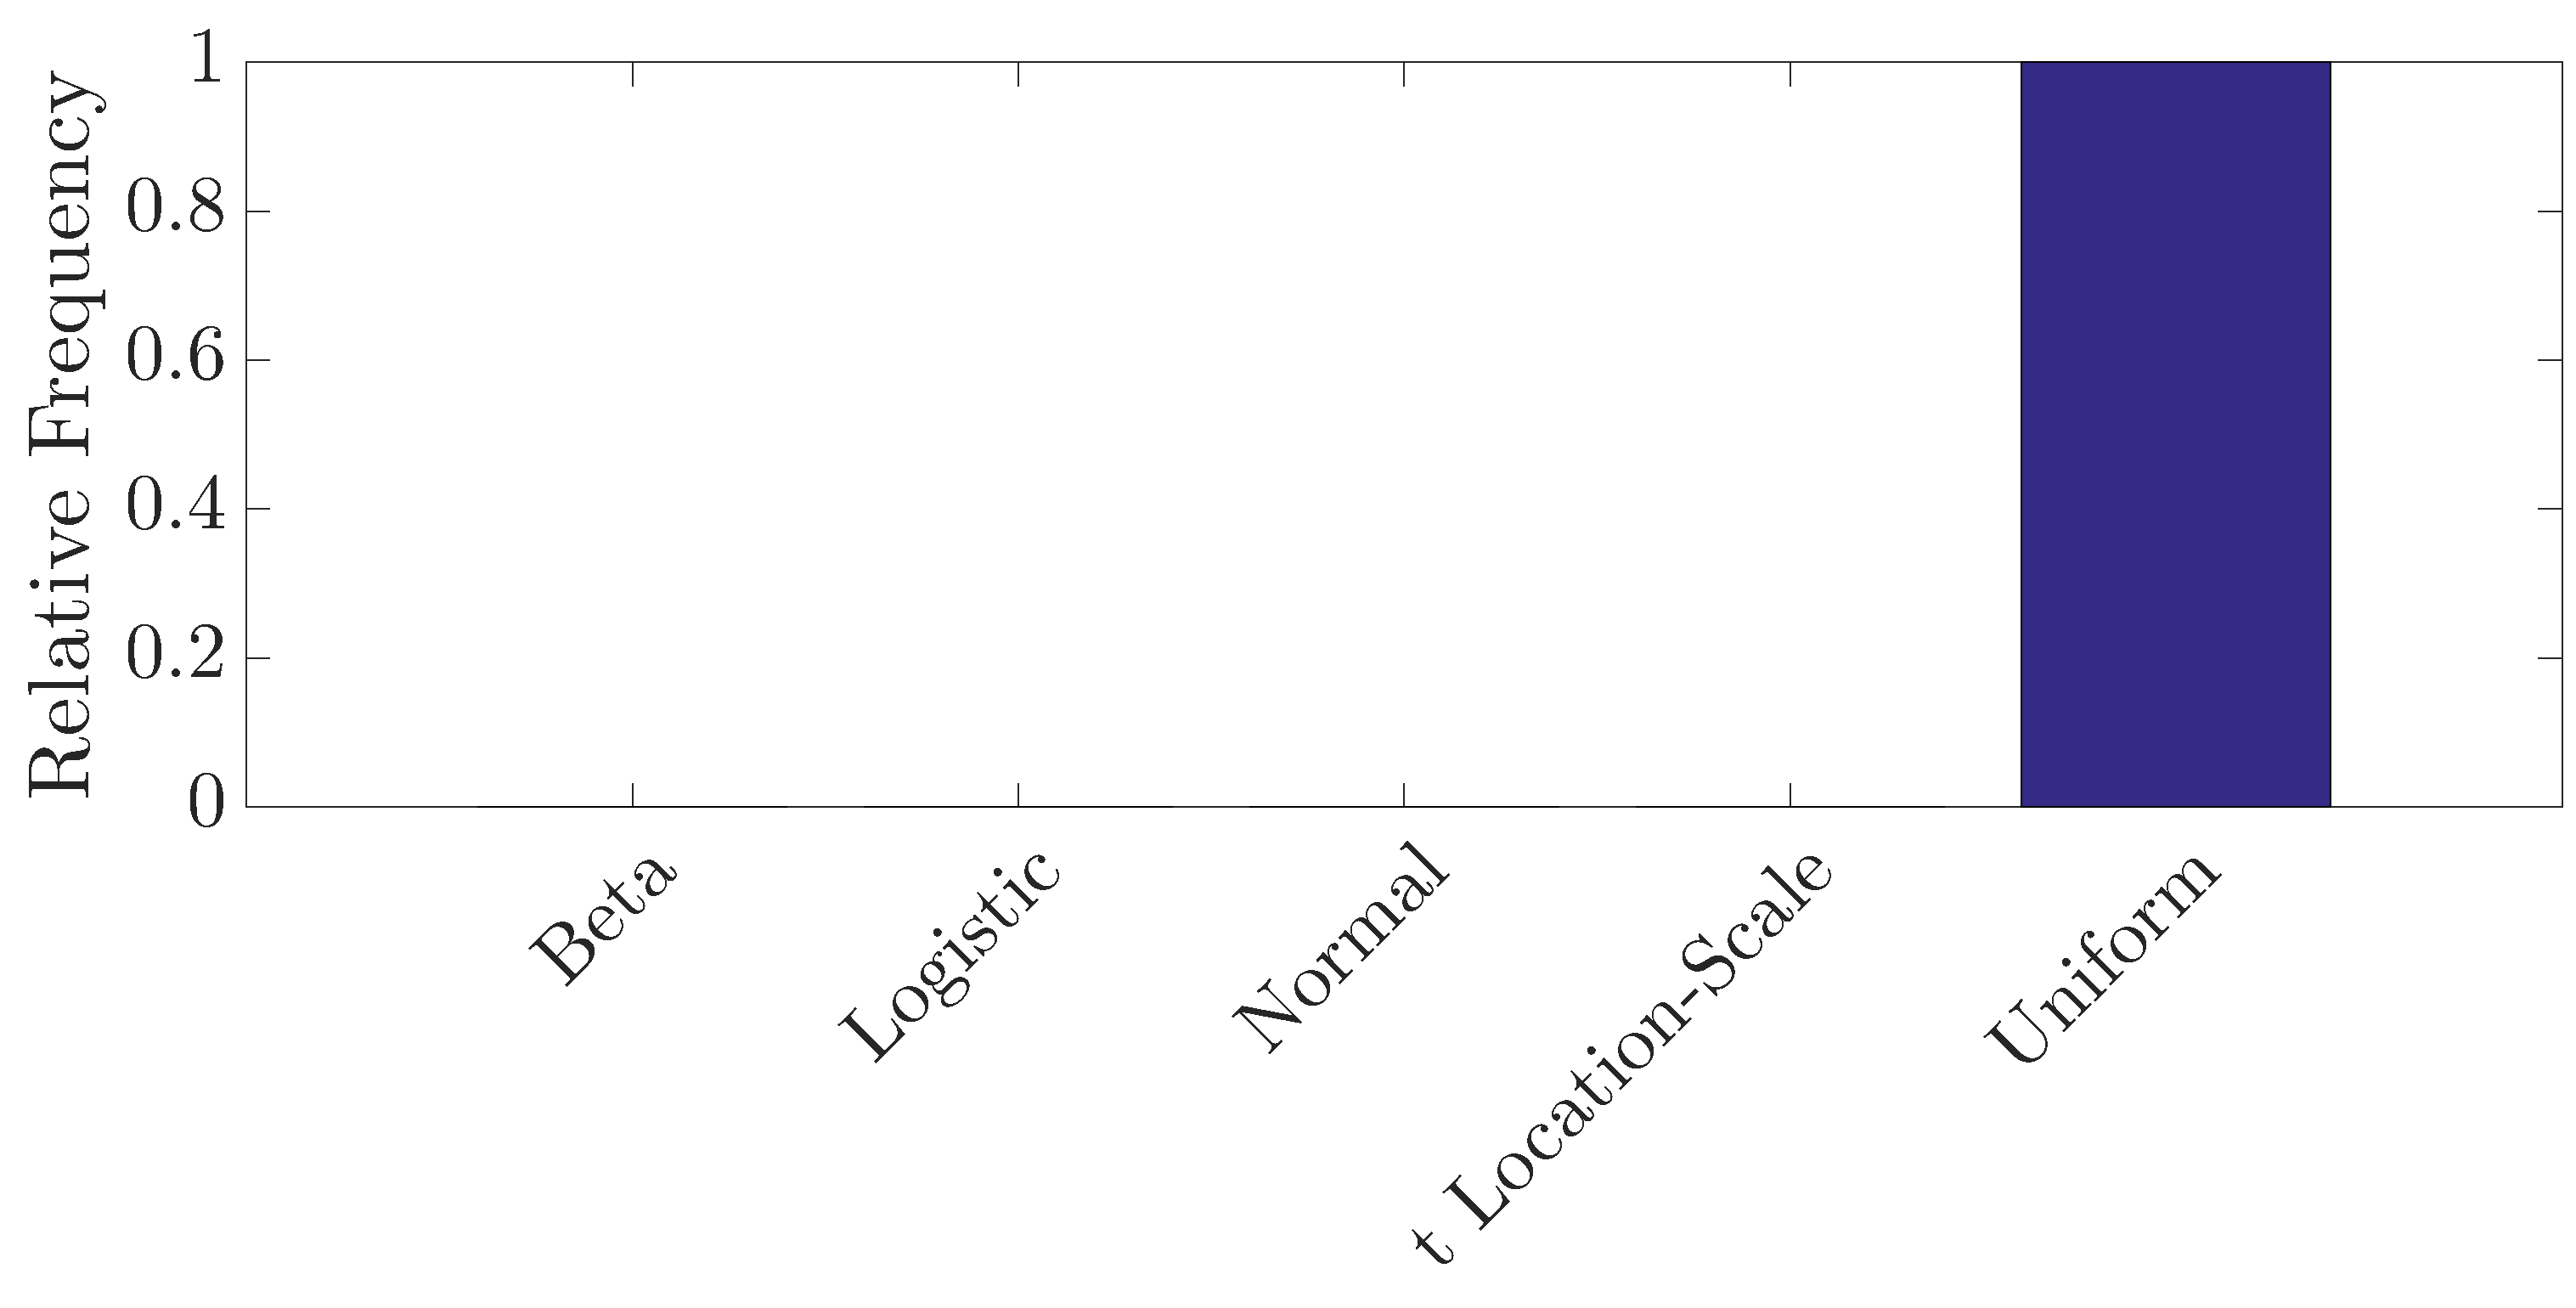
\includegraphics[width=0.49\textwidth]{images/Phase_percent.eps}
%	\caption{The relative frequency associated with the chosen statistical distribution that best models \ac{CFR} phase in accord with the adopted criteria.}
%	\label{Phase_percent}
%\end{figure}
%
%\begin{figure}[h!]
%	\centering
%	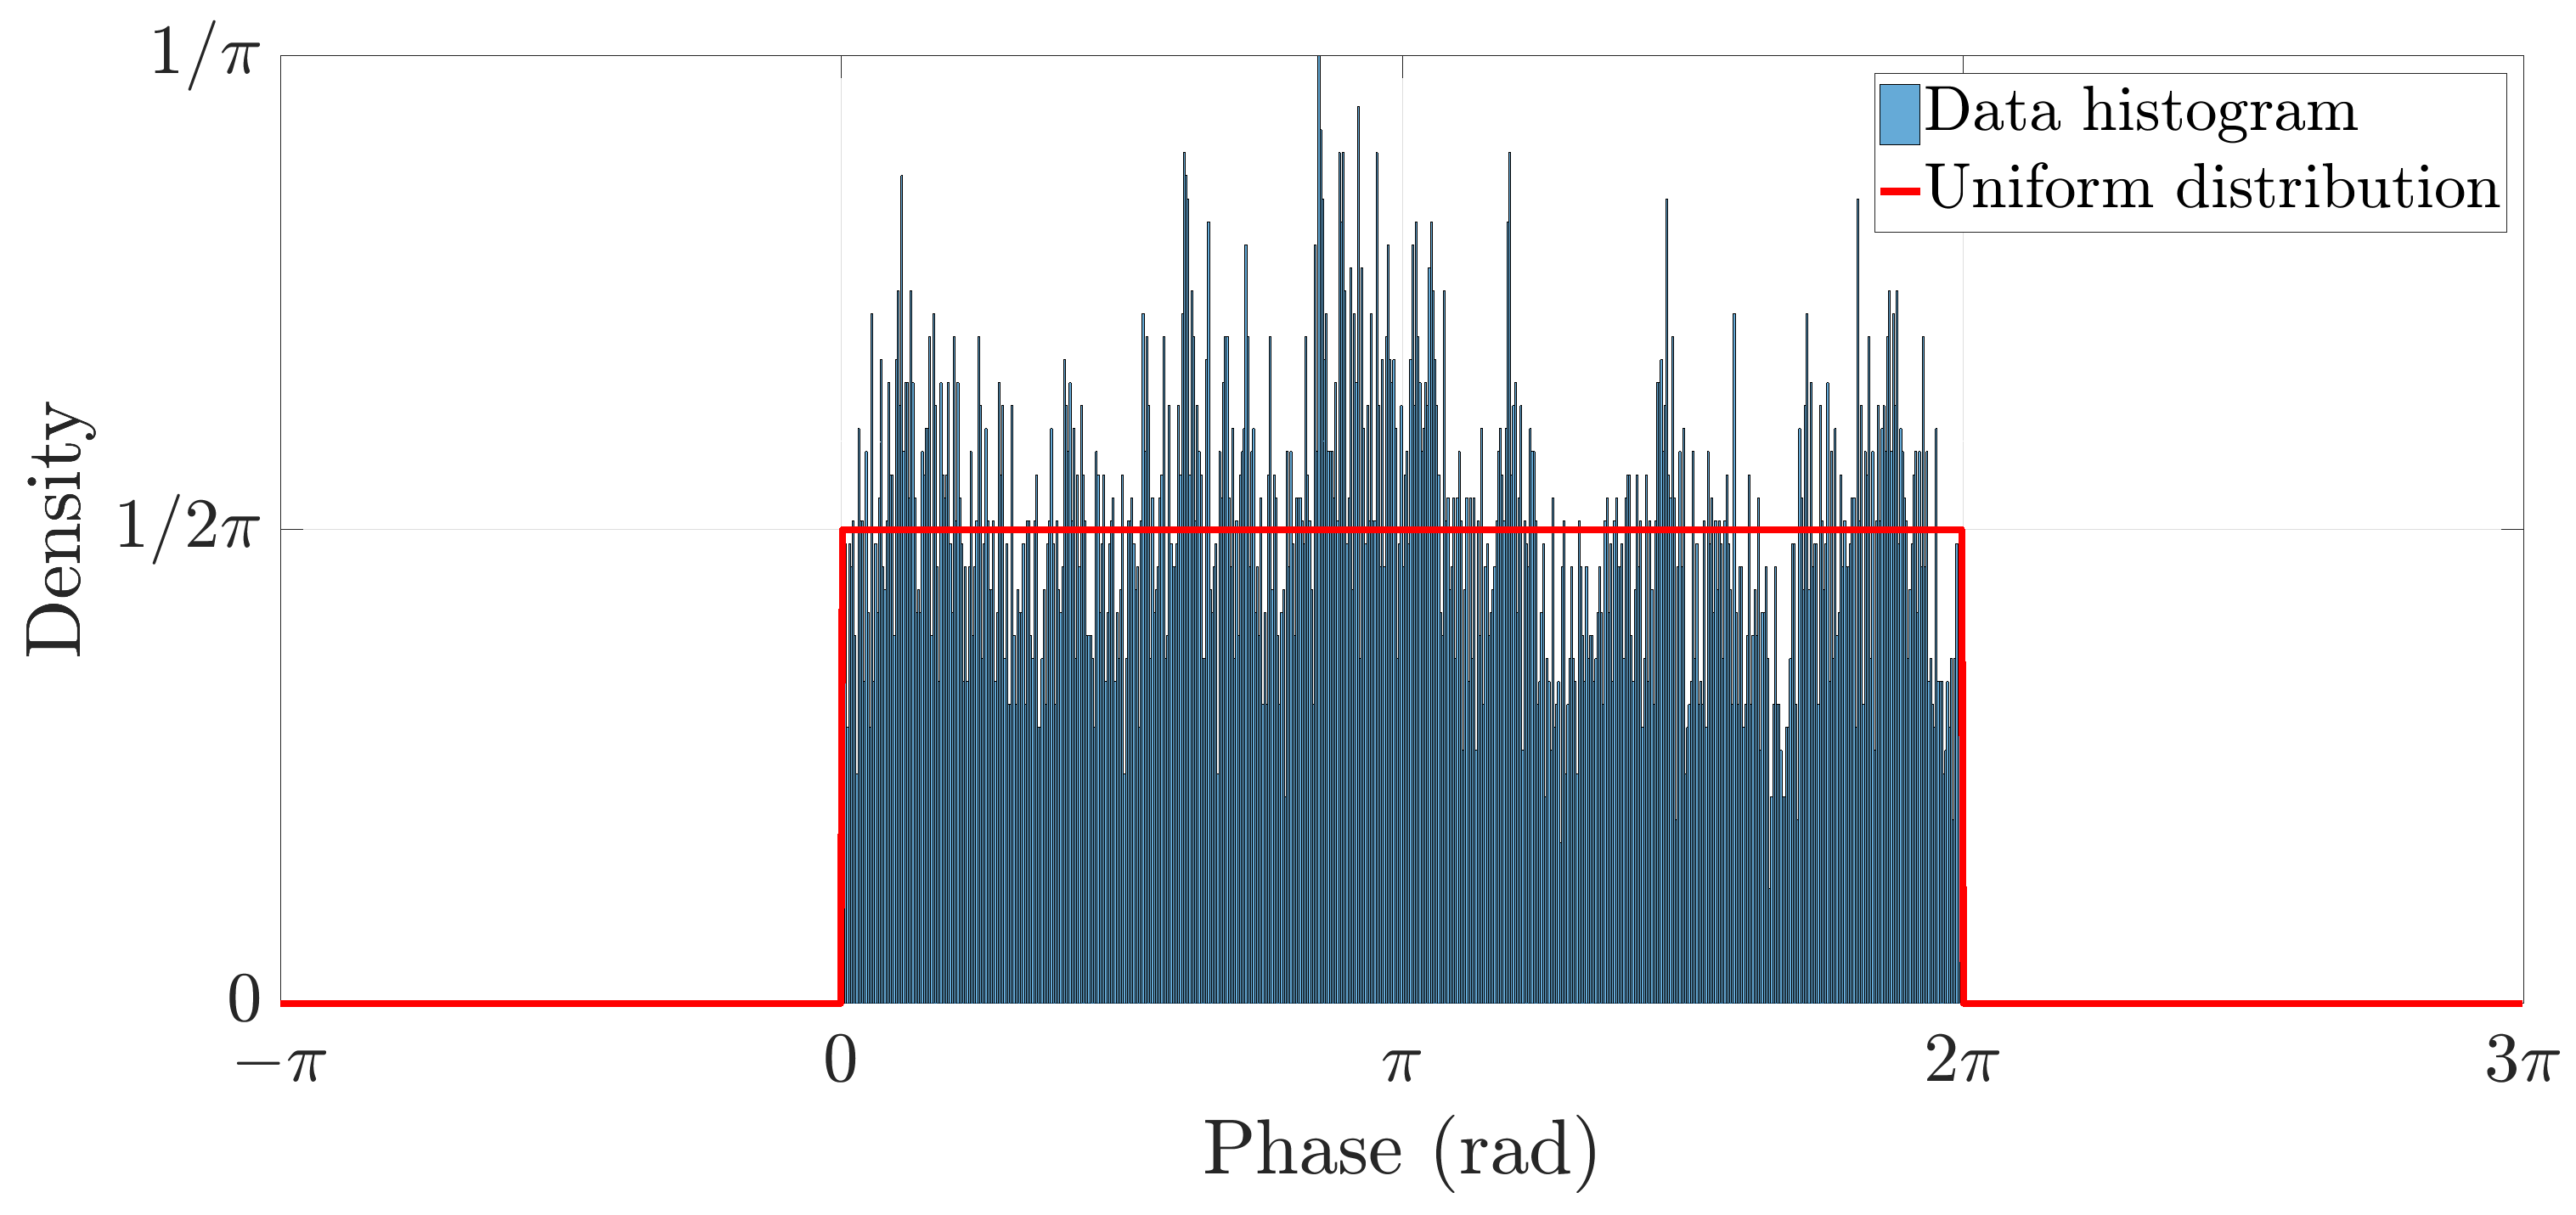
\includegraphics[width=0.49\textwidth]{images/Phase_hist.eps}
%	\caption{The relative frequency of the phase of the valid \ac{CFR} estimates at the sample $k$ = 1067 ($k\Delta f= 52.1$ MHz) using the Uniform distribution.}
%	\label{phase_example}
%\end{figure}
%
%\begin{figure}[h!]
%	\centering
%	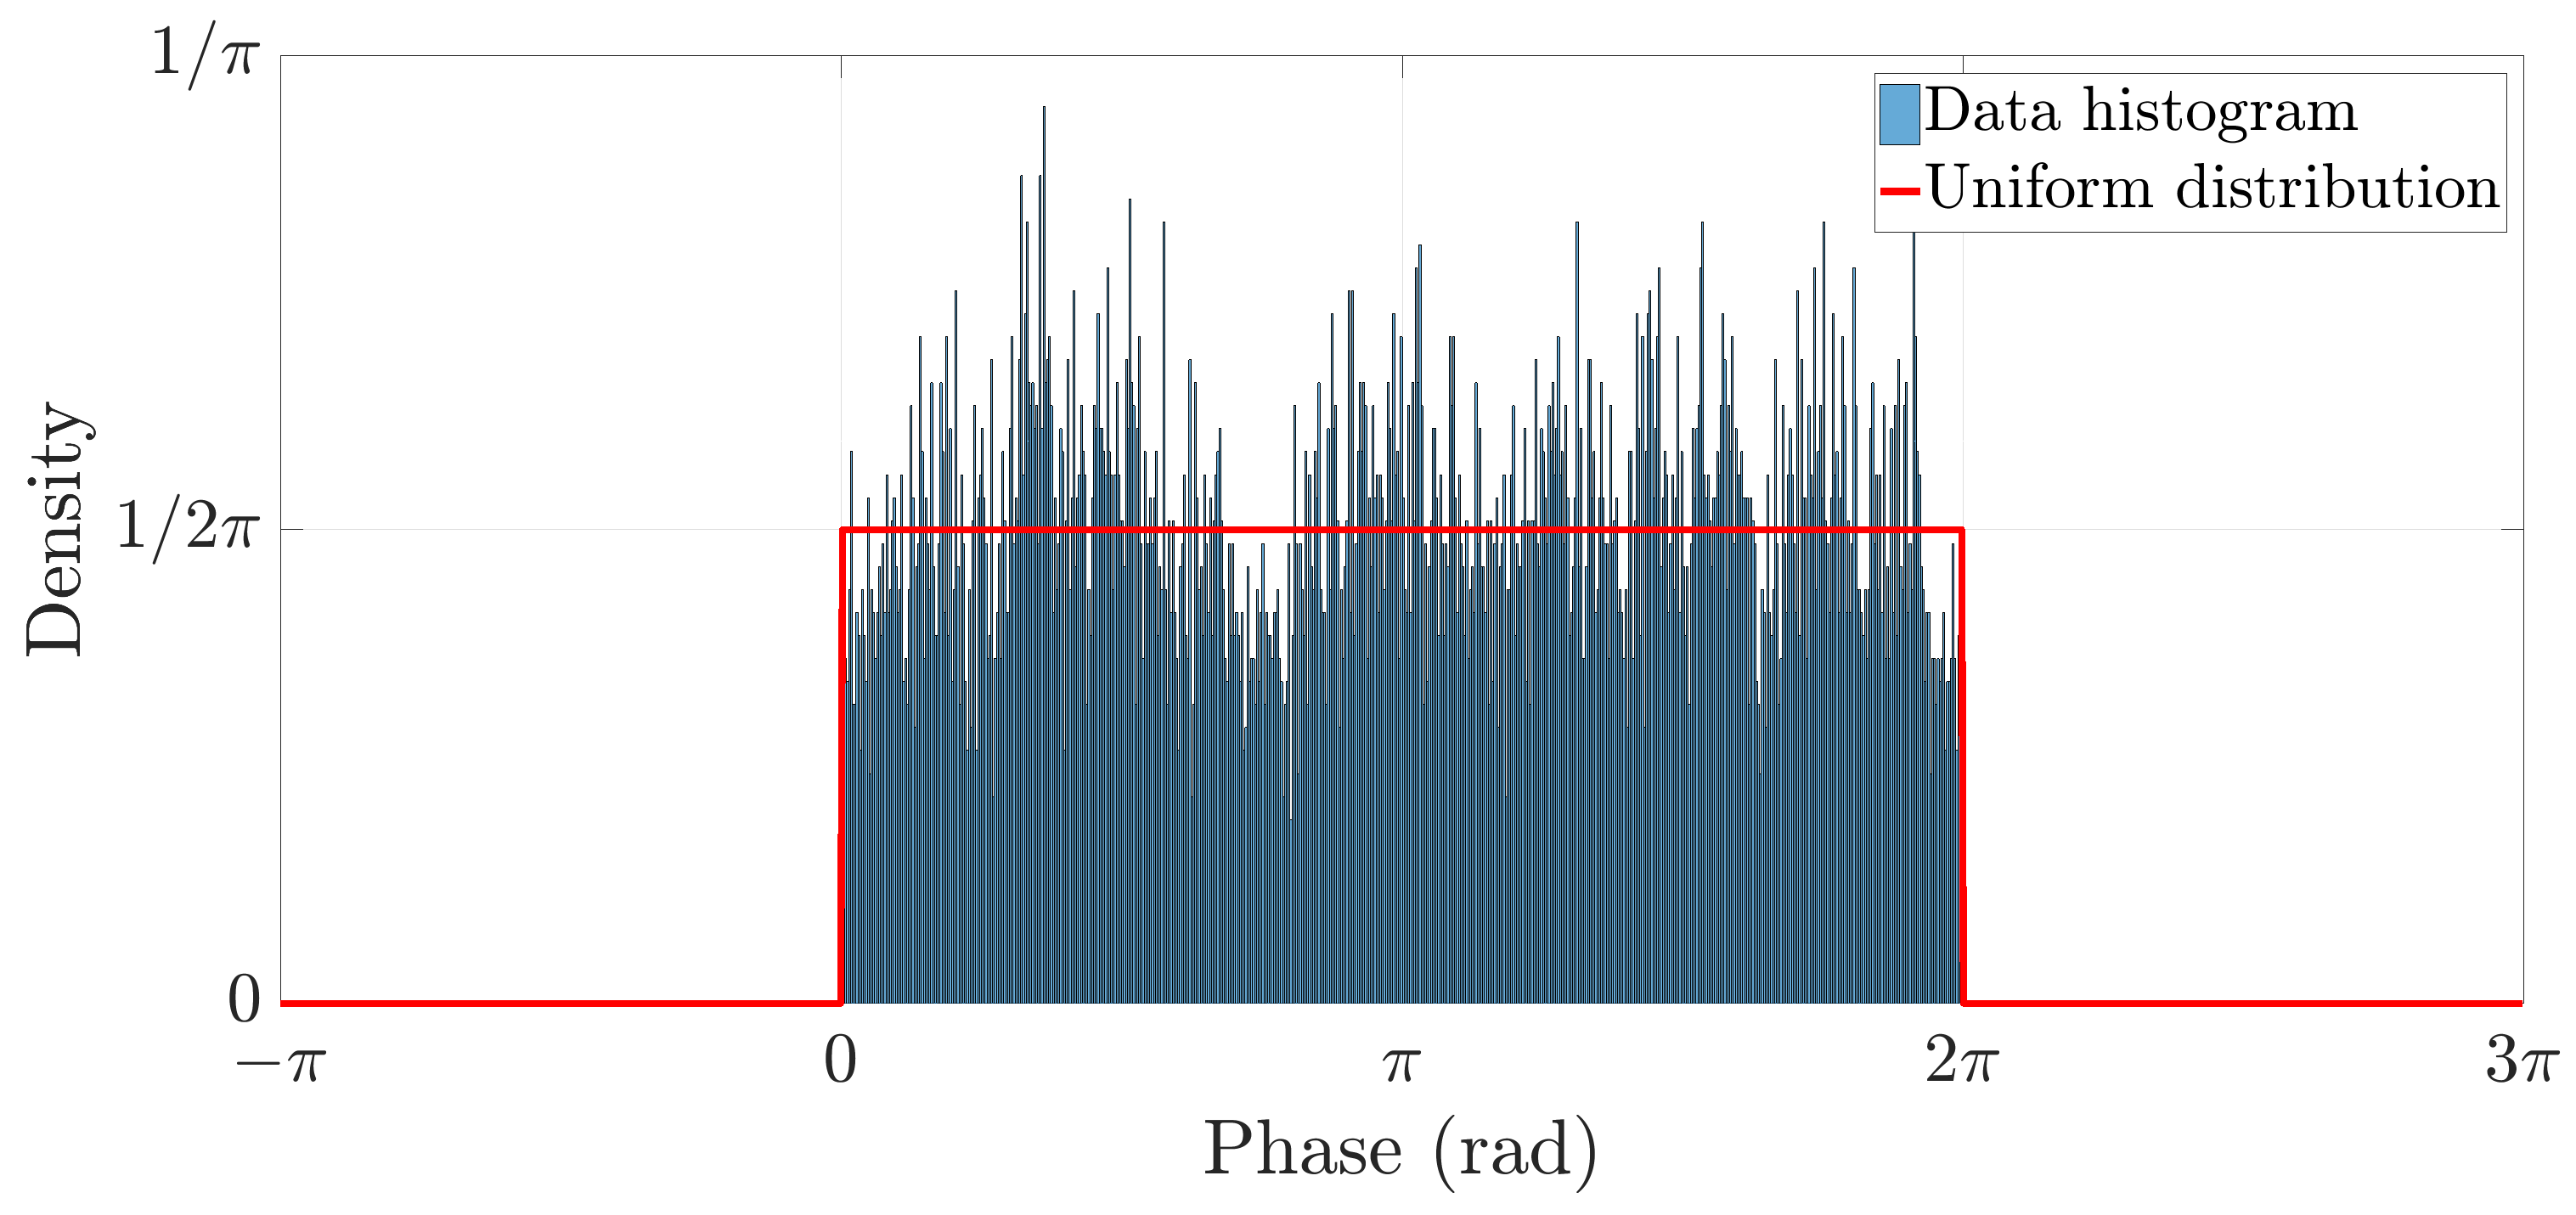
\includegraphics[width=0.49\textwidth]{images/Phase_hist2.eps}
%	\caption{The relative frequency of the phase of the valid \ac{CFR} estimates at the sample $k$ = 1600 ($k\Delta f= 78.125$ MHz) using the Uniform distribution.}
%	\label{phase_example2}
%\end{figure}

\section{Conclusions}
%This paper has presented a statistical characterization and modeling of the \ac{CFR} estimates of the Brazilian in-home \ac{PLC} channels, constituting an important result to support future efforts in simulating and designing in-home broadband \ac{PLC} systems. The statistical characterization and modeling have been based on the analysis of a data set of measured \ac{CFR} estimates, covering the frequency band between $1.7$ and $100$~MHz, acquired from a measurement campaign performed in seven typical Brazilian residences. This work has assumed the magnitude and phase of the \ac{CFR} estimates as two \acp{r.v.} ($|{\bf H}|$ and ${\bf \Theta}$).
% 
%We have obtained an uncorrelated statistical model for the two random processes. The magnitude of the \ac{CFR} estimates has been observed to be a non-stationary random process, modeled by the Beta distribution with parameter varying within the frequency  bandwidth. The use of the cubic Spline interpolation technique has allowed to obtain the parameter of the Beta distribution in the continuous-time domain. Also, we have shown that the phase of the \ac{CFR} estimates is a stationary random process with samples modeled by the Uniform distribution defined in $[0,2\pi]$ regardless of the frequency value.

\section*{Acknowledgements}
Authors acknowledge financial support from CNPq, CAPES, FAPEMIG, Smarti9 LTD. and INERGE.

\bibliographystyle{IEEEtran}
\bibliography{Ref}

%\begin{IEEEbiography}{Thiago Nogueira}
%Biography text here.
%\end{IEEEbiography}

\end{document}